\chapter{Arhitektura i dizajn sustava}
		
			\normalfont{Prilikom izrade naše aplikacije morali smo odlučiti kako ćemo najbolje organizirati aplikaciju tako da više klijenata može istodobno pristupati našoj stranici. Odabrali smo model mrežne aplikacije klijent – poslužitelj(server). Poslužitelj je aplikacija koja nudi uslugu, u našem slučaju nudi mogućnost pretraživanje zabavnih sadržaja. Kada stigne zahtjev, ona šalje odgovor.
			Klijent je aplikacija koja traži uslugu, u našem slučaju to su svi korisnici. Ona pošalje zahtjev i čeka na odgovor. Dakle, server ne pohranjuje podatke o klijentu, nego samo odgovara na upite klijenta. Protokol kojim se provodi komunikacija je HTTP.
				
		}
		
		\begin{figure}[h]
			\centering
			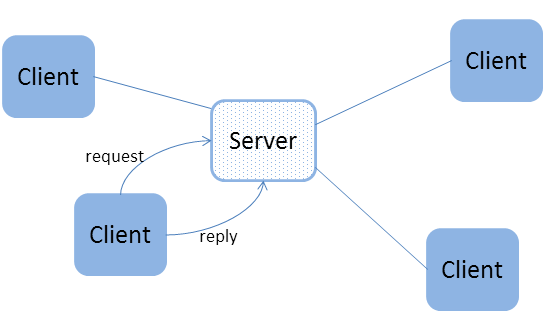
\includegraphics[width=\linewidth]{slike/klijent_server_model.PNG}
			\caption{Klijent-Server model}
			\label{fig:model1}
		\end{figure}
		
		\pagebreak
		
		\textbf{Backend dio aplikacije}
		
		\medskip
		
		\normalfont{Zbog dobre upoznatosti sa Javom, ali i velikog izbora mogućnosti koji nam nudi odabrali smo nju kao jezik za backend dio aplikacije. Uz to koristit ćemo i Spring Framework.}
		
		\normalfont\noindent{Web sloj će biti gornji sloj aplikacije. On je odgovoran za procesiranje korisnikovog unosa i vraćanja točnih informacija. On se također brine za greške koje bace drugi dijelovi aplikacije. Također to će nam biti prvi sloj da blokiramo korisnike koji žele napasti našu aplikaciju.}
		
		\normalfont\noindent{Servisni sloj sjedi iza web sloja. On se ponaša kao transakcijska granica te sadrži i servise aplikacije i infrastrukture. Odgovoran je za autorizaciju. On sadrži kod koji komunicria sa vanjskim resursima kao što su datotečni sustav, databaza ili email servisi..}
		
		\normalfont\noindent{Repozitorni sloj služi za komunikaciju sa bazom podataka.}
		
		\bigskip
		
		\begin{figure}[h]
			\centering
			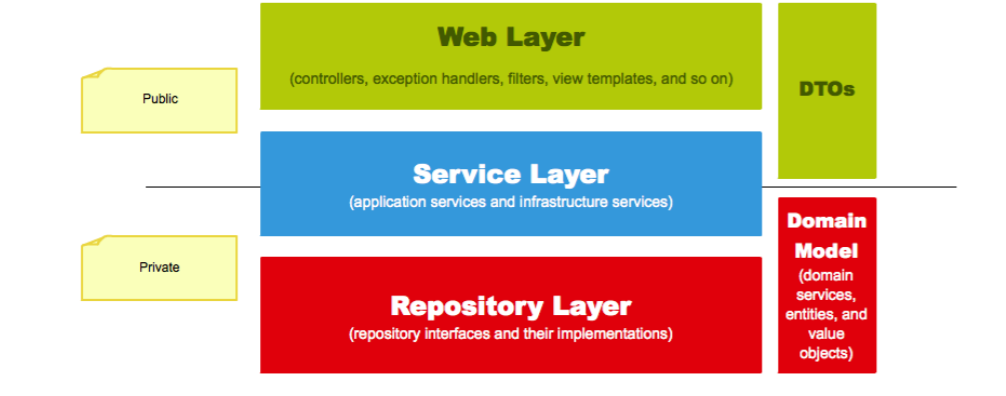
\includegraphics[width=\linewidth]{slike/arhitektura_springa.png}
			\caption{Spring arhitektura}
			\label{fig:arh1}
		\end{figure}
	
		\pagebreak
		
		\normalfont{Ovdje je slika kako bi to sve trebalo biti povezano u cjelinu. Koristimo poznatu dakle Spring MVC arhitekturu. MVC je skraćenica od Model, View, Controller. U kraćim crtama, nakon što dobijemo zahtjev koji dođe do našeg kontrolera, stvaramo model na osnovu podataka iz baze te osnovu njega i odgovora generiranog iz kontorlera stvara se odgovor, VIEW, kod nas JSP datoteke stvara se odgovor. JSP označava Java Server Page, stranicu koja generira html te se na taj način korisniku stvara odgovor.}
		
		\begin{figure}[h]
			\centering
			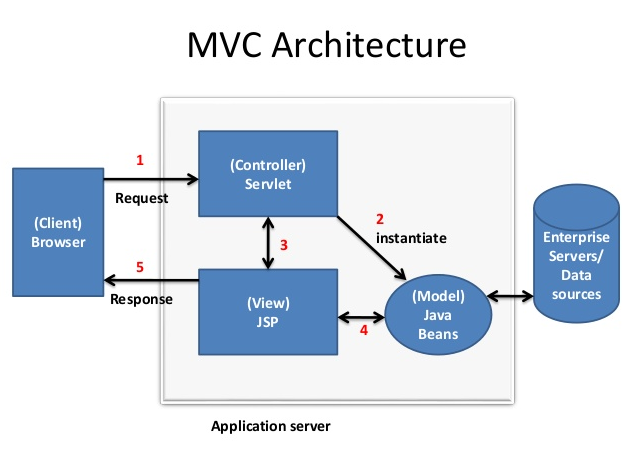
\includegraphics[width=\linewidth]{slike/mvc_arhitektura.png}
			\caption{MVC arhitektura}
			\label{fig:arh2}
		\end{figure}
	
		\pagebreak
		
		\textbf{Frontend dio aplikacije}
		
		\medskip
		
		\normalfont{Kako je spomenuto već za frontend dio aplikacije koristimo se JSP tehnologijom. U JSP datoteci mi dobivamo model na osnovu kojeg se generiraju komponente i dakle cijela stranica. Ona stvara odgovor i generira HTML, a izgled komponente je realiziran uporabom CSS jezika.}
		
		\normalfont\noindent{Za dizajn ćemo iskoristiti Bootstrap modul koji sadrži niz već gotovih dizajniranih komponenti kako bi to bilo što je moguće oku ljepše.U web poslužitelju nalaze se naše JSP datoteke. 
		}
	
		\begin{figure}[h]
			\centering
			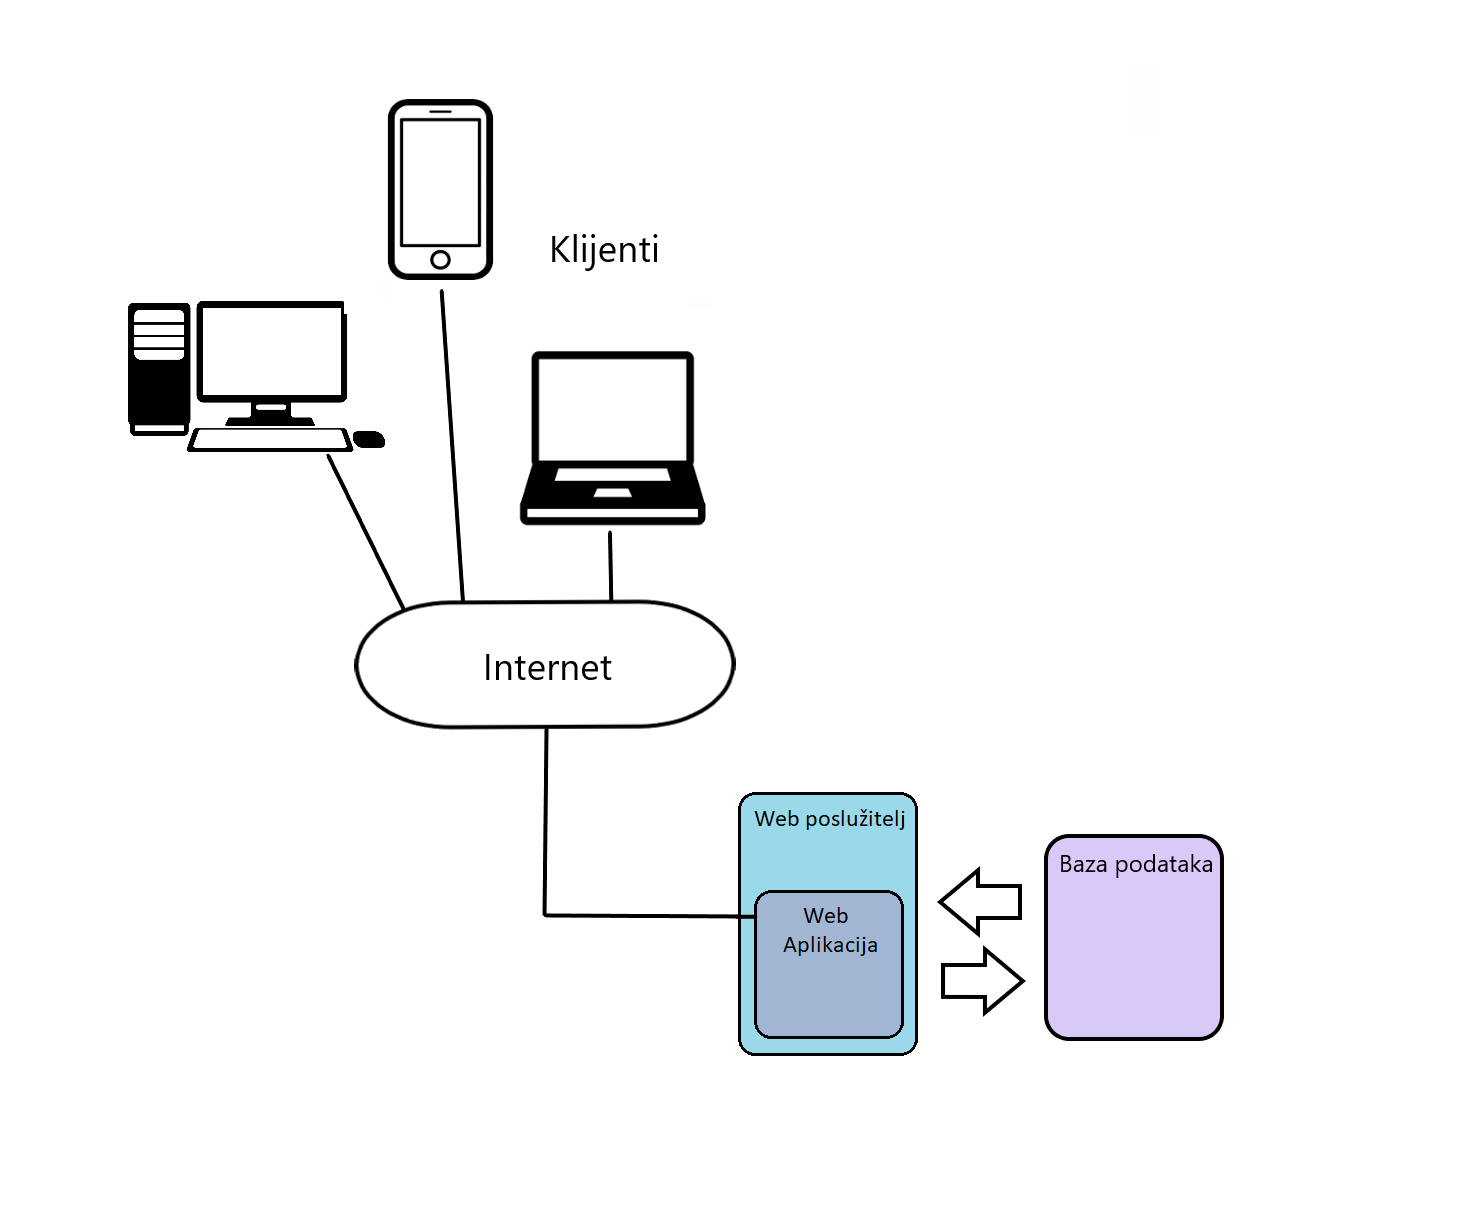
\includegraphics[width=\linewidth]{slike/jsp_arh.png}
			\caption{JSP arhitektura}
			\label{fig:arh3}
		\end{figure}	
		
		\pagebreak
				
		\section{Baza podataka}
	
	Za potrebe našeg sustava koristit ćemo relacijsku bazu podataka koja svojom strukturom olakšava modeliranje stvarnog svijeta. Gradivna jedinka baze je relacija, odnosno tablica koja je definirana svojim imenom i skupom atributa. Zadaća baze podataka je brza i jednostavna pohrana, izmjena i dohvat podataka za daljnju obradu.
	Baza podataka ove aplikacije sastoji se od sljedećih entiteta: 
	
	\begin{packed_item}
		
		\item  Korisnik
		\item  Posjetitelj
		\item  Kartica
		\item  PayPal
		\item  Organizator
		\item  Događaj
		\item  Kategorija
		\item  Kategorija i događaj
		\item  Slika
		\item  Video
		\item  Recenzija
		\item  Interes
		\item  Vrsta interesa
		\item  Područje obavijesti
		\item  Kategorija obavijesti
		\item  Područje
	\end{packed_item}
	
	
	
		\subsection{Opis tablica}
	
	
	
	
	\textbf{Korisnik}  \ \ Ovaj entitet sadržava sve važne informacije o korisniku aplikacije. Sadrži atribute: korisnik\_id, email, password\_hash, full\_name te vrsta\_korisnika. Ovaj entitet preko user\_id u vezi je \textit{One-to-One} s entitetima Posjetitelj, Organizator i Administrator.
	
	\begin{longtabu} to \textwidth {|X[10, l]|X[6, l]|X[20, l]|}
		
		\hline \multicolumn{3}{|c|}{\textbf{Korisnik}}	 \\[3pt] \hline
		\endfirsthead
		
		\hline \multicolumn{3}{|c|}{\textbf{Korisnik}}	 \\[3pt] \hline
		\endhead
		
		\hline 
		\endlastfoot
		
		\cellcolor{yellow}Korisnik\_ID & INT	&  jedinstveni identifikator korisnika 	\\ \hline
		Email	& VARCHAR &  e-mail adresa korisnika 	\\ \hline 
		Password\_Hash & VARCHAR &  hash lozinke \\ \hline 
		Full\_Name & VARCHAR	&  	ime i prezime korisnika	\\ \hline 
		Vrsta\_korisnika	& VARCHAR & razina ovlasti korisnika  	\\ \hline 
		
		
	\end{longtabu}
	
	
	
	\textbf{Posjetitelj}  \ \ Ovaj entitet sadržava sve važne informacije o posjetitelju. Sadrži atribute: user\_id, nick i obavijest\_id.  Ovaj entitet preko user\_id u vezi je \textit{One-to-One} s entitetom Korisnik, \textit{One-to-Many} s entitetom Recenzija, \textit{One-to-Many} s entitetom Interes, \textit{One-to-Many} s entitetom ObavijestPodručje, \textit{One-to-Many} s entitetom ObavijestKategorija.
	
	\begin{longtabu} to \textwidth {|X[7, l]|X[6, l]|X[20, l]|}
		
		\hline \multicolumn{3}{|c|}{\textbf{Posjetitelj}}	 \\[3pt] \hline
		\endfirsthead
		
		\hline \multicolumn{3}{|c|}{\textbf{Posjetitelj}}	 \\[3pt] \hline
		\endhead
		
		\hline 
		\endlastfoot
		
		\cellcolor{green}Korisnik\_ID & INT	&  	jedinstveni identifikator korisnika 	\\ \hline
		\cellcolor{LightBlue}Nick	& VARCHAR &  korisničko ime posjetitelja 	\\ \hline 
		\cellcolor{LightBlue}Obavijest\_ID	& VARCHAR &  jedinstveni identifikator obavijesti 	\\ \hline 
		
		
		
		
	\end{longtabu}
	
	\textbf{Administrator}  \ \ Ovaj entitet sadržava sve važne informacije o administratoru. Sadrži atribute: user\_id i pretplata.  Ovaj entitet preko korisnik\_id u vezi je \textit{One-to-One} s entitetom Korisnik.
	
	\begin{longtabu} to \textwidth {|X[7, l]|X[6, l]|X[20, l]|}
		
		\hline \multicolumn{3}{|c|}{\textbf{Administrator}}	 \\[3pt] \hline
		\endfirsthead
		
		\hline \multicolumn{3}{|c|}{\textbf{Administrator}}	 \\[3pt] \hline
		\endhead
		
		\hline 
		\endlastfoot
		
		\cellcolor{green}Korisnik\_ID & INT	&  	jedinstveni identifikator korisnika 	\\ \hline
		\cellcolor{LightBlue}Pretplata	& VARCHAR &  pretplaćeni događaji 	\\ \hline 
		
		
		
		
		
	\end{longtabu}
	
	
	
	
	
	
	\textbf{Organizator}  \ \ Ovaj entitet sadržava sve važne informacije o organizatoru. Sadrži atribute: korisnik\_id, fizička\_adresa, web\_adresa, kartica\_id, račun\_vrijedi\_do i paypal\_id. Ovaj entitet preko user\_id u vezi je \textit{One-to-One} s entitetom Korisnik, \textit{One-to-Many} s entitetom Dogadaj, preko kartica\_id i korisnik\_id u vezi je \textit{Many-to-One} s entitetom Kartica te preko paypal\_id u vezi je \textit{Many-to-One} s entitetom PayPal.
	
	\begin{longtabu} to \textwidth {|X[8, l]|X[6, l]|X[20, l]|}
		
		\hline \multicolumn{3}{|c|}{\textbf{Organizator}}	 \\[3pt] \hline
		\endfirsthead
		
		\hline \multicolumn{3}{|c|}{\textbf{Organizator}}	 \\[3pt] \hline
		\endhead
		
		\hline 
		\endlastfoot
		
		\cellcolor{green}Korisnik\_ID & INT	&  jedinstveni identifikator korisnika 	\\ \hline
		\cellcolor{green}Račun\_vrijedi\_do & TIMESTAMP	&  rok trajanja korisničkog računa 	\\ \hline
		Fizicka\_adresa	& VARCHAR &   adresa stanovanja	\\ \hline 
		Web\_adresa & VARCHAR	&  direktna poveznica na vlastitu web stranicu		\\ \hline 
		\cellcolor{green}Kartica\_ID & INT	&  	jedinstveni identifikator kreditne kartice 	\\ \hline
		\cellcolor{LightBlue}PayPal\_ID	& INT &  jedinstveni identifikator PayPal računa 	\\ \hline 
		
		
		
	\end{longtabu}
	
	
	
	\textbf{Kartica}  \ \ Ovaj entitet sadržava sve važne informacije o kartici. Sadrži atribute: kartica\_id, korisnik\_id i broj\_kartice.  Ovaj entitet preko kartica\_id u vezi je \textit{One-to-Many} s entitetom Organizator. 
	
	\begin{longtabu} to \textwidth {|X[7, l]|X[6, l]|X[20, l]|}
		
		\hline \multicolumn{3}{|c|}{\textbf{Kartica}}	 \\[3pt] \hline
		\endfirsthead
		
		\hline \multicolumn{3}{|c|}{\textbf{Kartica}}	 \\[3pt] \hline
		\endhead
		
		\hline 
		\endlastfoot
		
		\cellcolor{green}Kartica\_ID & INT	&  	jedinstveni identifikator kartice 	\\ \hline
		\cellcolor{LightBlue}Broj\_Kartice	& VARCHAR &  broj kartice 	\\ \hline 
		\cellcolor{LightBlue}Korisnik\_ID	& INT &  jedinstveni identifikator korisnika 	\\ \hline 
		
		
		
		
	\end{longtabu}
	
	
	
	\textbf{PayPal}  \ \ Ovaj entitet sadržava sve važne informacije o PayPalu-u. Sadrži atribute: paypal\_id i paypal\_email.  Ovaj entitet preko paypal\_id u vezi je \textit{One-to-Many} s entitetom Organizator.
	
	\begin{longtabu} to \textwidth {|X[7, l]|X[6, l]|X[20, l]|}
		
		\hline \multicolumn{3}{|c|}{\textbf{PayPal}}	 \\[3pt] \hline
		\endfirsthead
		
		\hline \multicolumn{3}{|c|}{\textbf{PayPal}}	 \\[3pt] \hline
		\endhead
		
		\hline 
		\endlastfoot
		
		\cellcolor{green}PayPal\_ID & INT	&  	jedinstveni identifikator PayPal računa 	\\ \hline
		PayPal\_Mail	& VARCHAR &  PayPal adresa 	\\ \hline 
		
		
		
		
	\end{longtabu}
	
	
	
	\textbf{Događaj}  \ \ Ovaj entitet sadržava sve važne informacije o događajima. Sadrži atribute: događaj\_id, naziv događaja, lokacija, područje\_id, vrijeme\_početka, vrijeme\_završetka, kategorija\_id, opis\_događaja i korisnik\_id. Ovaj entitet preko kategorija\_id u vezi je \textit{One-to-Many} s entitetom Kategorija, \textit{One-to-Many} s entitetom SlikaDogađaj, \textit{One-to-Many} s entitetom VideoDogađaj, \textit{One-to-Many} s entitetom Recenzija, \textit{One-to-Many} s entitetom Interes te preko korisnik\_id \textit{Many-to-One} s entitetom Organizator.
	
	\begin{longtabu} to \textwidth {|X[8, l]|X[6, l]|X[20, l]|}
		
		\hline \multicolumn{3}{|c|}{\textbf{Događaj}}	 \\[3pt] \hline
		\endfirsthead
		
		\hline \multicolumn{3}{|c|}{\textbf{Događaj}}	 \\[3pt] \hline
		\endhead
		
		\hline 
		\endlastfoot
		
		\cellcolor{yellow}Događaj\_ID & INT	&  	jedinstveni identifikator događaja	\\ \hline
		Naziv\_događaja & VARCHAR &  naziv događaja \\ \hline 
		Lokacija	& VARCHAR &  lokacija događaja 	\\ \hline 
		\cellcolor{green}Podrucje\_ID & INT	&  	jedinstveni identifikator područja	\\ \hline 
		Vrijeme\_početka & TIMESTAMP	&  	vrijeme početka događaja	\\ \hline 
		Vrijeme\_završetka & TIMESTAMP	&  vrijeme završetka događaja		\\ \hline 
		\cellcolor{yellow}Korisnik\_ID & INT	&  	jedinstveni identifikator organizatora	\\ \hline
		\cellcolor{yellow}Kategorija\_ID & INT	&  	jedinstveni identifikator kategorije	\\ \hline
		\cellcolor{yellow}Opis\_događaja & Varchar	&  	opis događaja	\\ \hline
		
	\end{longtabu}
	
	
	
	\textbf{Kategorija}  \ \ Ovaj entitet sadržava sve važne informacije o događajima. Sadrži atribute: kategorija\_id i naziv\_kategorije. Ovaj entitet preko kategorija\_id u vezi je \textit{One-to-Many} s entitetom Događaj i u vezi \textit{One-to-Many} s entitetom ObavijestKategorija.
	
	\begin{longtabu} to \textwidth {|X[8, l]|X[6, l]|X[20, l]|}
		
		\hline \multicolumn{3}{|c|}{\textbf{Kategorija}}	 \\[3pt] \hline
		\endfirsthead
		
		\hline \multicolumn{3}{|c|}{\textbf{Kategorija}}	 \\[3pt] \hline
		\endhead
		
		\hline 
		\endlastfoot
		
		\cellcolor{yellow}Kategorija\_ID & INT	&  	jedinstveni identifikator kategorije	\\ \hline
		Naziv\_Kategorije & VARCHAR &  naziv kategorije \\ \hline 
		
		
		
	\end{longtabu}
	
	
	
	
	
	\textbf{Slika}  \ \ Ovaj entitet sadržava sve važne informacije o slikama. Sadrži atribute: slika\_id i događaj\_id.  Ovaj entitet preko dogadaj\_id u vezi je \textit{Many-to-One} s entitetom SlikaDogađaj.
	
	\begin{longtabu} to \textwidth {|X[8, l]|X[6, l]|X[20, l]|}
		
		\hline \multicolumn{3}{|c|}{\textbf{Slika}}	 \\[3pt] \hline
		\endfirsthead
		
		\hline \multicolumn{3}{|c|}{\textbf{Slika}}	 \\[3pt] \hline
		\endhead
		
		\hline 
		\endlastfoot
		
		\cellcolor{yellow}Slika\_ID & INT	&  	jedinstveni identifikator slike	\\ \hline
		\cellcolor{green} Naziv\_slika & VARCHAR & naziv slike \\ \hline 
		
		
		
		
	\end{longtabu}
	
	\textbf{SlikaDogađaj}  \ \ Ovaj entitet sadržava sve važne informacije o slikama. Sadrži atribute: slika\_id i događaj\_id.  Ovaj entitet preko dogadaj\_id u vezi je \textit{Many-to-One} s entitetom Događaj te \textit{Many-to-One} vezi s entitetom Slika.
	
	\begin{longtabu} to \textwidth {|X[8, l]|X[6, l]|X[20, l]|}
		
		\hline \multicolumn{3}{|c|}{\textbf{SlikaDogađaj}}	 \\[3pt] \hline
		\endfirsthead
		
		\hline \multicolumn{3}{|c|}{\textbf{SlikaDogađaj}}	 \\[3pt] \hline
		\endhead
		
		\hline 
		\endlastfoot
		
		\cellcolor{yellow}Slika\_ID & INT	&  	jedinstveni identifikator slike	\\ \hline
		\cellcolor{green} Dogadaj\_ID & INT & jedinstveni identifikator događaja \\ \hline 
		
		
		
		
	\end{longtabu}
	
	
	
	
	\textbf{Video}  \ \ Ovaj entitet sadržava sve važne informacije o videima. Sadrži atribute: video\_id i događaj\_id. Ovaj entitet preko dogadaj\_id u vezi je \textit{Many-to-One} s entitetom VideoDogađaj.
	
	\begin{longtabu} to \textwidth {|X[8, l]|X[6, l]|X[20, l]|}
		
		\hline \multicolumn{3}{|c|}{\textbf{Video}}	 \\[3pt] \hline
		\endfirsthead
		
		\hline \multicolumn{3}{|c|}{\textbf{Video}}	 \\[3pt] \hline
		\endhead
		
		\hline 
		\endlastfoot
		
		\cellcolor{yellow}Video\_ID & INT	&  	jedinstveni identifikator videa	\\ \hline
		\cellcolor{green} Naziv\_videa & VARCHAR & naziv videa \\ \hline 
		
		
		
	\end{longtabu}
	
	\textbf{VideoDogađaj}  \ \ Ovaj entitet sadržava sve važne informacije o videima. Sadrži atribute: video\_id i događaj\_id. Ovaj entitet preko dogadaj\_id u vezi je \textit{Many-to-One} s entitetom Događaj te \textit{Many-to-One} s entitetom Video.
	
	\begin{longtabu} to \textwidth {|X[8, l]|X[6, l]|X[20, l]|}
		
		\hline \multicolumn{3}{|c|}{\textbf{VideoDogađaj}}	 \\[3pt] \hline
		\endfirsthead
		
		\hline \multicolumn{3}{|c|}{\textbf{VideoDogađaj}}	 \\[3pt] \hline
		\endhead
		
		\hline 
		\endlastfoot
		
		\cellcolor{yellow}Video\_ID & INT	&  	jedinstveni identifikator videa	\\ \hline
		\cellcolor{green} Dogadaj\_ID & INT & jedinstveni identifikator događaja \\ \hline 
		
		
		
	\end{longtabu}
	
	
	
	
	
	
	
	\textbf{Recenzija}  \ \ Ovaj entitet sadržava sve važne informacije o recenzijama. Sadrži atribute: događaj\_id, korisnik\_id, tekst, datum\_stvaranja i naslov\_recenzije.
	Ovaj entitet preko dogadaj\_id u vezi je \textit{Many-to-One} s entitetom Dogadaj te preko korisnik\_id u vezi je \textit{Many-to-One} s entitetom Posjetitelj.
	
	\begin{longtabu} to \textwidth {|X[8, l]|X[6, l]|X[20, l]|}
		
		\hline \multicolumn{3}{|c|}{\textbf{Recenzija}}	 \\[3pt] \hline
		\endfirsthead
		
		\hline \multicolumn{3}{|c|}{\textbf{Recenzija}}	 \\[3pt] \hline
		\endhead
		
		\hline 
		\endlastfoot
		
		\cellcolor{green}Dogadaj\_ID & INT	&  	jedinstveni identifikator događaja	\\ \hline
		\cellcolor{green}Korisnik\_ID & INT & jedinstveni identifikator korisnika \\ \hline 
		Tekst	& VARCHAR &  tekst recenzije 	\\ \hline 
		Datum\_Stvaranja & TIMESTAP	&  	vrijeme objavljivanja recenzije	\\ \hline 
		Naslov\_recenzije & VARCHAR	&  	naslov recenzije	\\ \hline 
		
		
	\end{longtabu}
	
	
	
	\textbf{Interes}  \ \ Ovaj entitet sadržava sve važne informacije o interesima. Sadrži atribute: događaj\_id, korisnik\_id i interes\_id. Ovaj entitet preko dogadaj\_id u vezi je \textit{Many-to-One} s entitetom Dogadaj, preko korisnik\_id u vezi je \textit{Many-to-One} s entitetom Posjetitelj te preko interes\_id u vezi je \textit{Many-to-One} s entitetom VrstaInteresa.
	
	\begin{longtabu} to \textwidth {|X[8, l]|X[6, l]|X[20, l]|}
		
		\hline \multicolumn{3}{|c|}{\textbf{Interes}}	 \\[3pt] \hline
		\endfirsthead
		
		\hline \multicolumn{3}{|c|}{\textbf{Interes}}	 \\[3pt] \hline
		\endhead
		
		\hline 
		\endlastfoot
		
		\cellcolor{green}Korisnik\_ID & INT & jedinstveni identifikator korisnika \\ \hline 
		\cellcolor{green}Dogadaj\_ID & INT	&  	jedinstveni identifikatorr događaja	\\ \hline
		\cellcolor{green}Interes\_ID & INT & jedinstveni identifikator interesa \\ \hline 
		
		
	\end{longtabu}
	
	
	
	
	\textbf{Vrsta interesa}  \ \ Ovaj entitet sadržava sve važne informacije o vrstama interesa. Sadrži atribute: interes\_id i naziv\_interesa. Ovaj entitet preko interes\_id u vezi je \textit{One-to-Many} s entitetom Interes.
	
	\begin{longtabu} to \textwidth {|X[8, l]|X[6, l]|X[20, l]|}
		
		\hline \multicolumn{3}{|c|}{\textbf{VrstaInteresa}}	 \\[3pt] \hline
		\endfirsthead
		
		\hline \multicolumn{3}{|c|}{\textbf{VrstaInteresa}}	 \\[3pt] \hline
		\endhead
		
		\hline 
		\endlastfoot
		
		\cellcolor{yellow}Interes\_ID & INT	&  	jedinstveni identifikator interesta	\\ \hline
		Naziv\_interesa	& VARCHAR &  naziv interesa 	\\ \hline 
		
		
	\end{longtabu}
	
	\textbf{Obavijest}  \ \ Ovaj entitet sadržava sve važne informacije o obavijestima. Sadrži atribute: obavijest\_id i korisnik\_id.  Ovaj entitet preko dogadaj\_id u vezi je \textit{Many-to-One} s entitetom Dogadaj.
	
	\begin{longtabu} to \textwidth {|X[8, l]|X[6, l]|X[20, l]|}
		
		\hline \multicolumn{3}{|c|}{\textbf{Obavijest}}	 \\[3pt] \hline
		\endfirsthead
		
		\hline \multicolumn{3}{|c|}{\textbf{Obavijest}}	 \\[3pt] \hline
		\endhead
		
		\hline 
		\endlastfoot
		
		\cellcolor{yellow}Obavjest\_ID & INT	&  	jedinstveni identifikator slike	\\ \hline
		\cellcolor{green} Korisnik\_ID & INT & jedinstveni identifikator događaja \\ \hline 
		
		
		
	\end{longtabu}
	
	
	
	\textbf{ObavijestPodručje}  \ \ Ovaj entitet sadržava sve važne informacije o obavijestima sa različitih područja. Sadrži atribute: korisnik\_id i područje\_id. Ovaj entitet preko korisnik\_id u vezi je \textit{Many-to-One} s entitetom Posjetitelj te preko podrucje\_id u vezi je \textit{Many-to-One} s entitetom Podrucje.
	
	\begin{longtabu} to \textwidth {|X[8, l]|X[6, l]|X[20, l]|}
		
		\hline \multicolumn{3}{|c|}{\textbf{ObavijestPodrucje}}	 \\[3pt] \hline
		\endfirsthead
		
		\hline \multicolumn{3}{|c|}{\textbf{ObavijestPodrucje}}	 \\[3pt] \hline
		\endhead
		
		\hline 
		\endlastfoot
		
		\cellcolor{green}Korisnik\_ID & INT	&  	jedinstveni identifikator korisnika	\\ \hline
		\cellcolor{green}Podrucje\_ID	& INT &  jedinstveni identifikator područja	\\ \hline 
		
		
	\end{longtabu}
	
	
	
	
	\textbf{ObavijestKategorija}  \ \ Ovaj entitet sadržava sve važne informacije o obavijestima kategorija. Sadrži atribute: korisnik\_id, kategorija\_id i obavijest\_id.  Ovaj entitet preko korisnik\_id u vezi je \textit{Many-to-One} s entitetom Posjetitelj te preko kategorija\_id u vezi je \textit{Many-to-One} s entitetom Kategorija.
	
	\begin{longtabu} to \textwidth {|X[8, l]|X[6, l]|X[20, l]|}
		
		\hline \multicolumn{3}{|c|}{\textbf{ObavijestKategorija}}	 \\[3pt] \hline
		\endfirsthead
		
		\hline \multicolumn{3}{|c|}{\textbf{ObavijestKategorija}}	 \\[3pt] \hline
		\endhead
		
		\hline 
		\endlastfoot
		
		\cellcolor{green}Kategorija\_ID	& INT &  jedinstveni identifikator kategorije	\\ \hline 
		\cellcolor{green}Obavijest\_ID	& INT &  jedinstveni identifikator obavijesti	\\ \hline 
		
		
	\end{longtabu}
	
	
	\textbf{Područje}  \ \ Ovaj entitet sadržava sve važne informacije o područjima. Sadrži atribute: podrucje\_id i naziv\_podrucje\_id.  Ovaj entitet preko podrucje\_id u vezi je \textit{One-to-Many} s entitetom ObavijestPodrucje i u vezi \textit{One-to-Many} s entitetom Dogadaj.
	
	\begin{longtabu} to \textwidth {|X[8, l]|X[6, l]|X[20, l]|}
		
		\hline \multicolumn{3}{|c|}{\textbf{Podrucje}}	 \\[3pt] \hline
		\endfirsthead
		
		\hline \multicolumn{3}{|c|}{\textbf{Podrucje}}	 \\[3pt] \hline
		\endhead
		
		\hline 
		\endlastfoot
		
		\cellcolor{yellow}Podrucje\_ID & INT	&  	jedinstveni identifikator korisnika	\\ \hline
		Naziv\_podrucja	& VARCHAR &  jedinstveni identifikator područja	\\ \hline 
		
		
	\end{longtabu}
	
	\subsection{Dijagram baze podataka}
	\begin{figure}[H]
		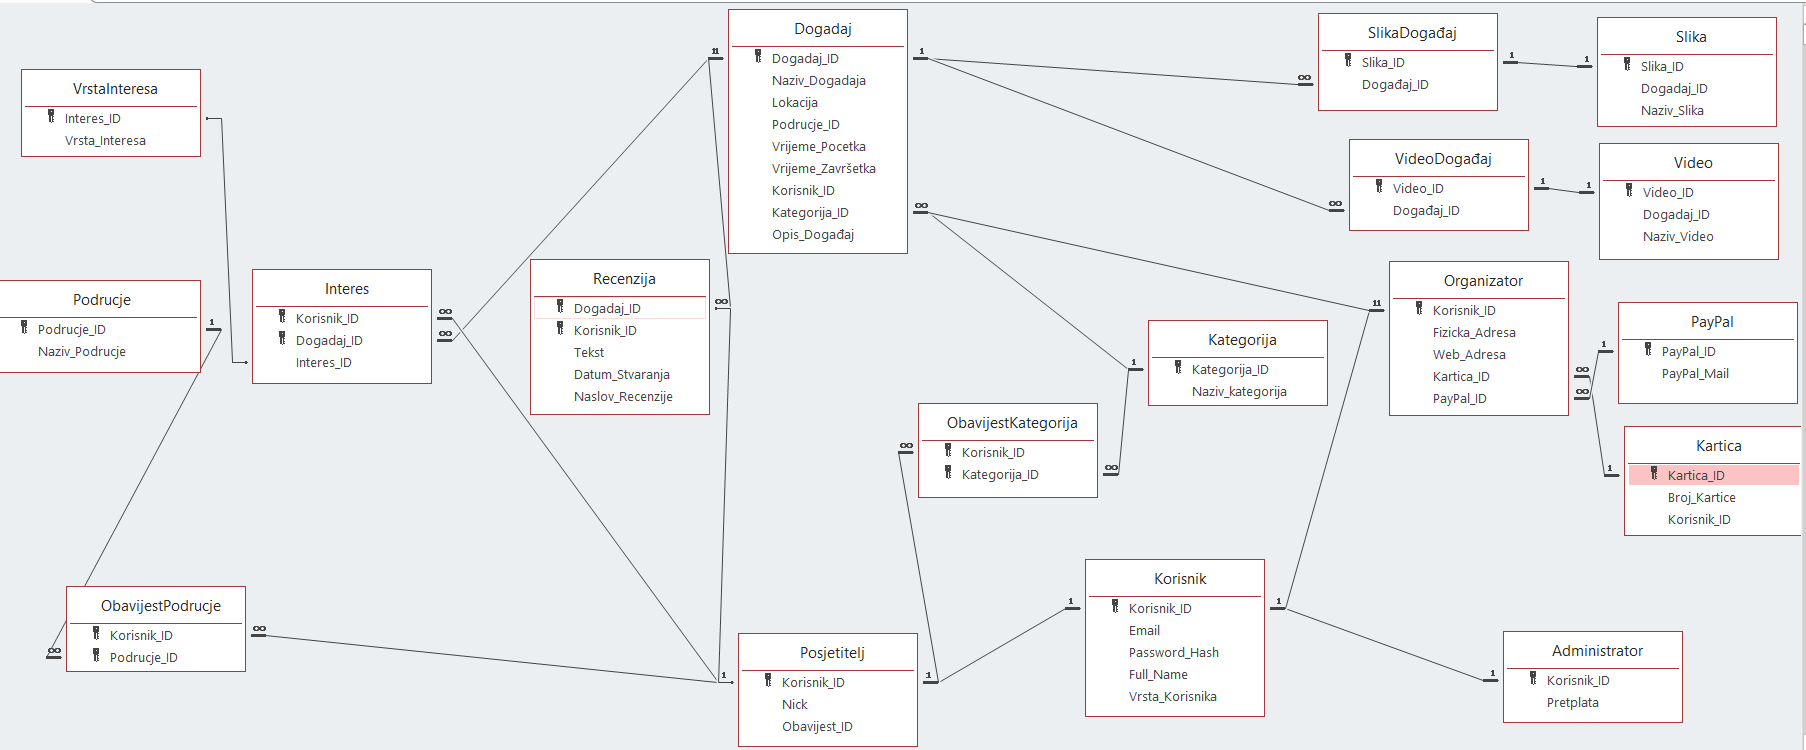
\includegraphics[scale=0.46]{slike/ERModel2.PNG}
		\centering
		\caption{E-R dijagram baze podataka}
		\label{fig:promjene}
	\end{figure}
	
	\eject
			
			
		\section{Dijagram razreda}
		
		\normalfont U našem sustavu postoje tri vrste korisnika: Admin, Organizator (Organiser) te Posjetitelj(Visitor).
		
		\normalfont\noindent Svaki od tih korisnika predstavlja jedan objekt koji nasljeđuje objekt User-a. U sustavu postoje događaji (Event)  koje može dodavati organizator, postoje recenzije (Review) koje može pisati prijavljeni posjetitelj, postoje interesi(Interest) koje može izraziti posjetitelj za određeni događaj. Kako postoje razne vrste interesa, dodali smo tu InterestType koji nam služi kao jedan od interesa. Uz to na svaki događaj mogu se dodati videi(Video) i slike (Picture) te događaj pripada određenoj kategoriji (Category) i području (Area).  Posjetitelji mogu postaviti obavijest (Notification) vezano za više područja te kategorija.
		
		\normalfont\noindent Organizator mora moći platiti članarinu koju postavlja admin, te ima mogućnost plaćanja Paypal-om (PayPal) ili kreditnom karticom(Credit Card).
		
		\normalfont\noindent našoj web aplikaciji poveznicu sa bazom podataka ostvarili smo preko Repostioryja. Svaki objekt ima svoj Repository, a svaki Service ima poveznicu na Repository.  Service nam služi kao objekt poveznica između Repositoryja i Controllera tako da imamo između dodatni nivo provjere podataka koji dolaze prema bazi podataka i odlaze prema Controllerima.\\
		
		
		\noindent Klijentske zahtjeve primaju Controlleri i oni obavljaju posao koji je potreban kako bi se prikazao sav sadržaj na stranici. U slučaju da je potrebno, oni vrše preusmjeravanje korisnika. Controlleri pripreme ono što će dalje JSP koristiti kako bi izgenerirao HTML sadržaj.
		
		\begin{figure}[H]
			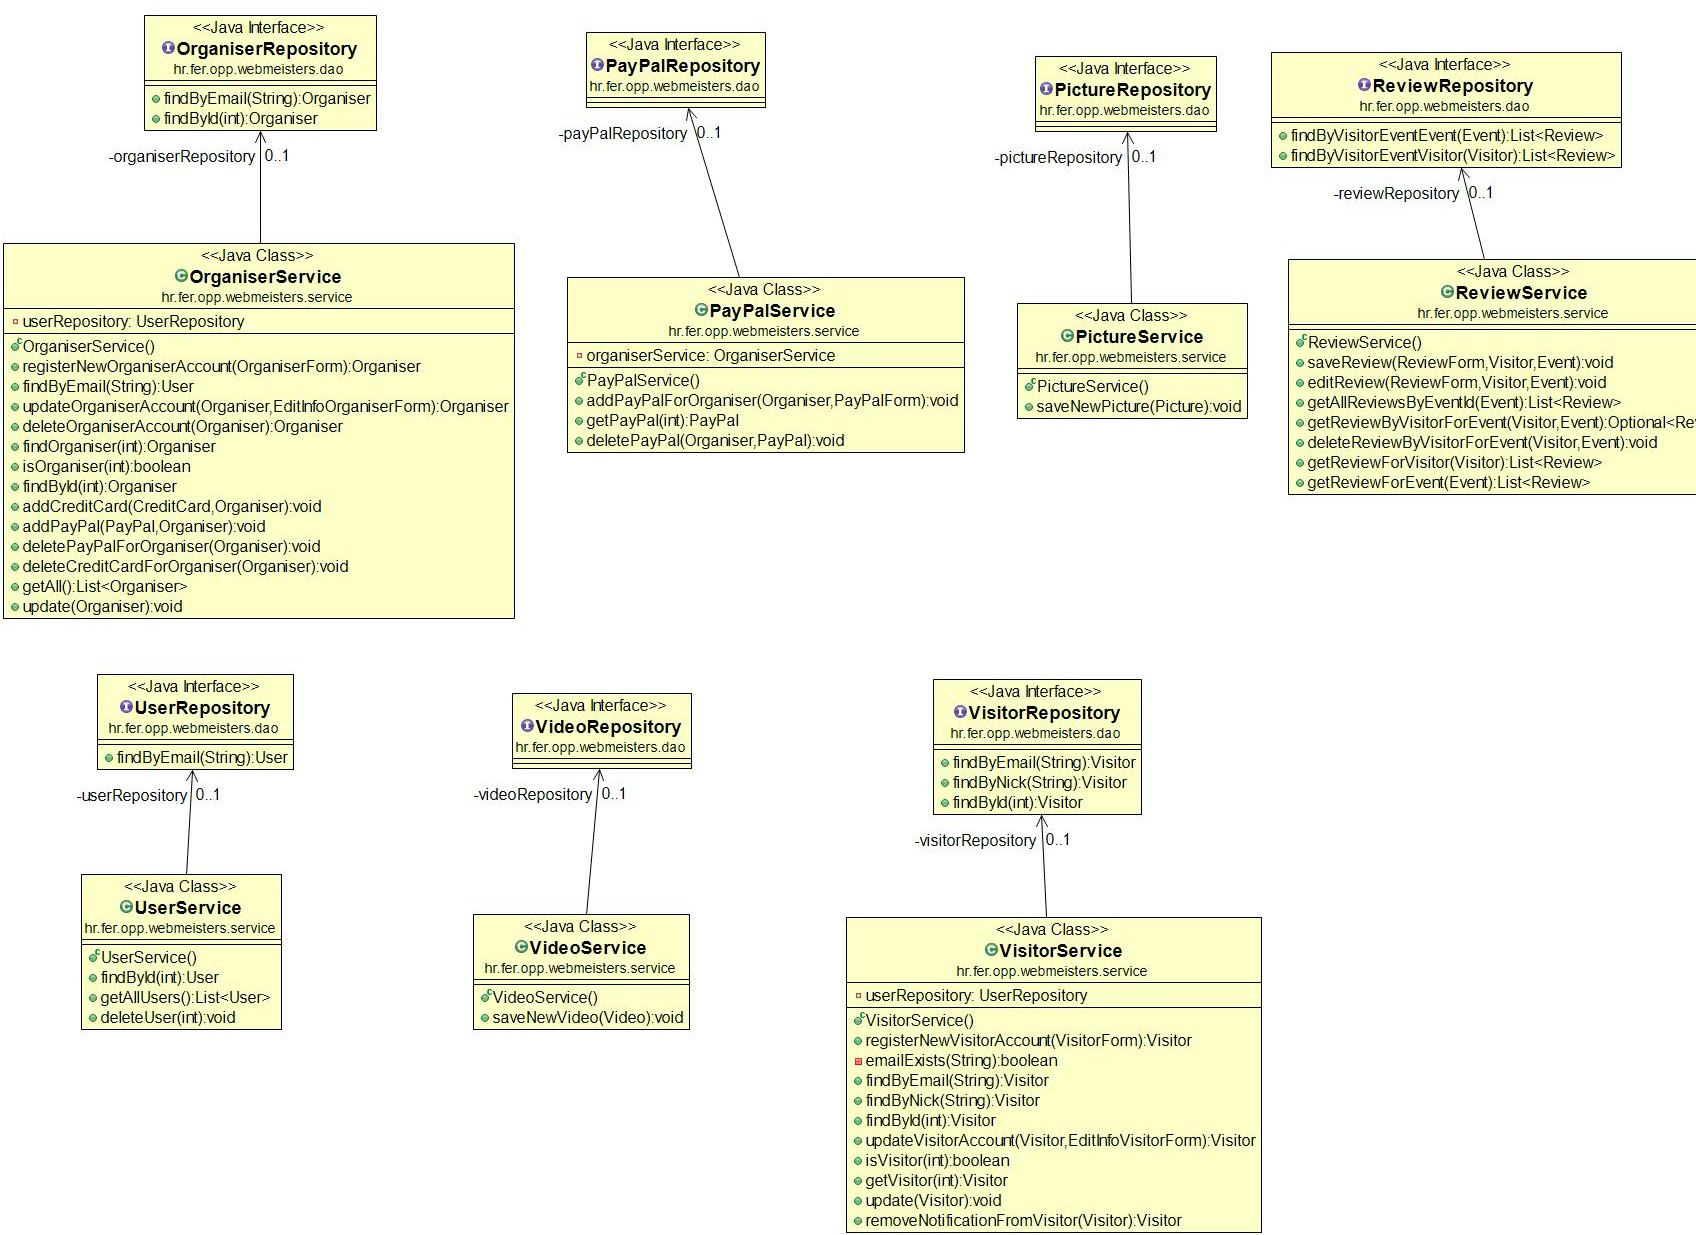
\includegraphics[scale=0.4]{slike/dijagram1a.jpg}
			\centering
			\caption{Prvi dio slike poveznice Servicea i Repositoryja}
			\label{fig:dijagramraz1}
		\end{figure}
	
		\begin{figure}[H]
			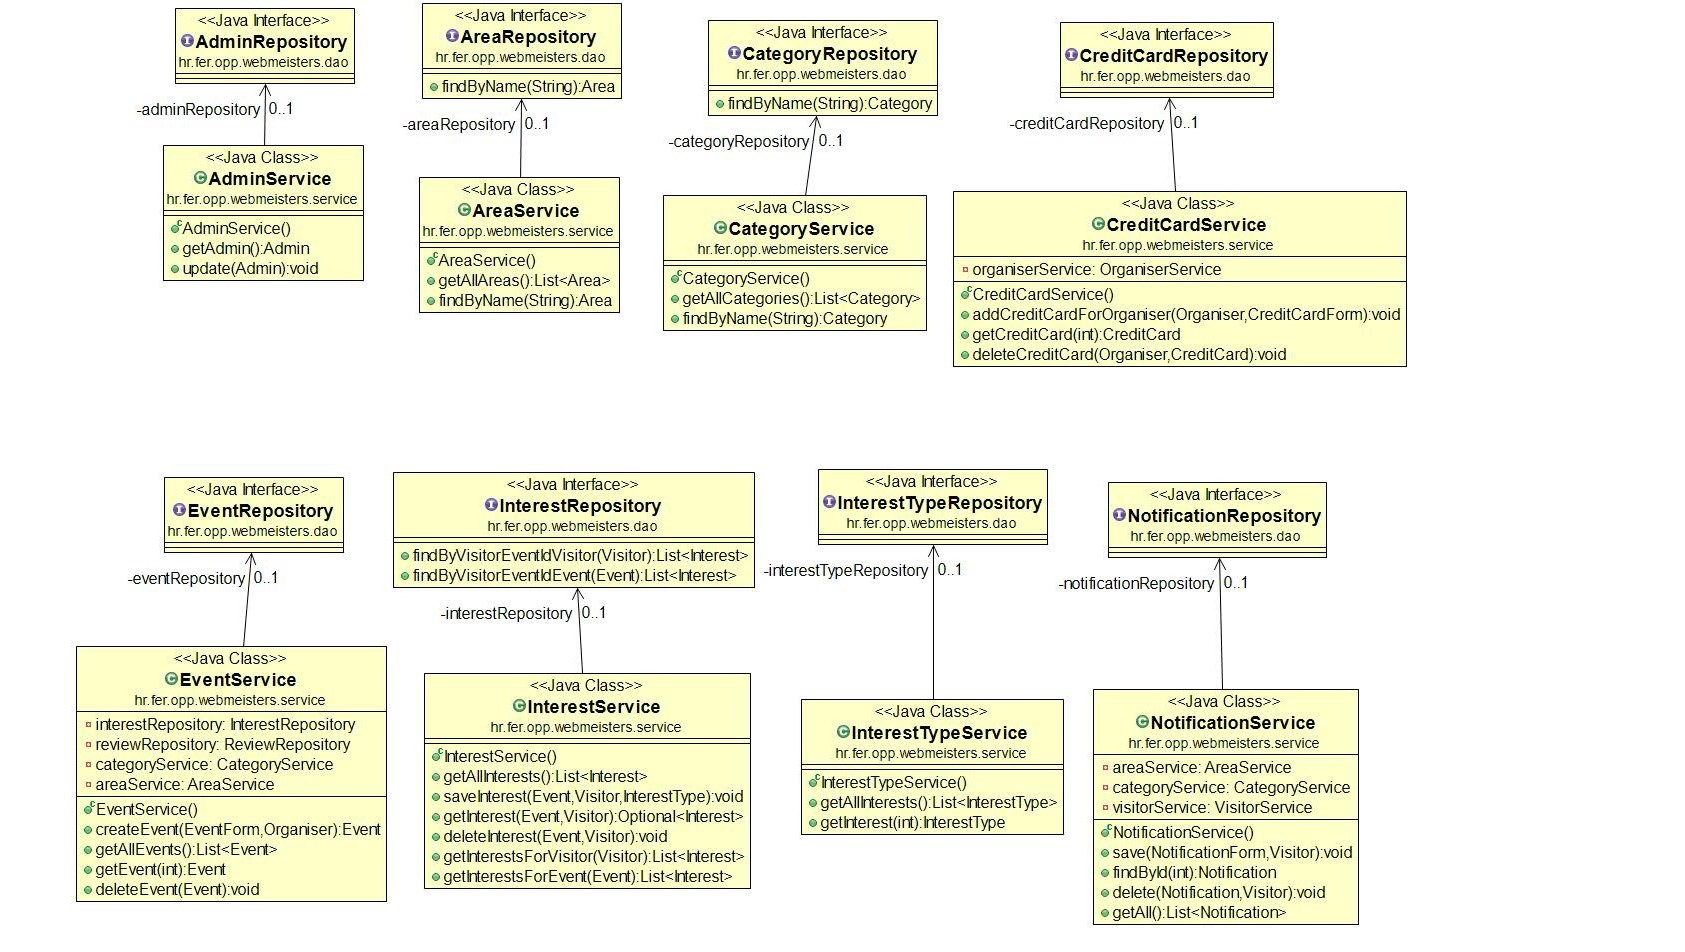
\includegraphics[scale=0.4]{slike/dijagram1b.jpg}
			\centering
			\caption{Drugi dio poveznica Servicea i Repositoryja}
			\label{fig:dijagramraz2}
		\end{figure}
	
		\begin{figure}[H]
			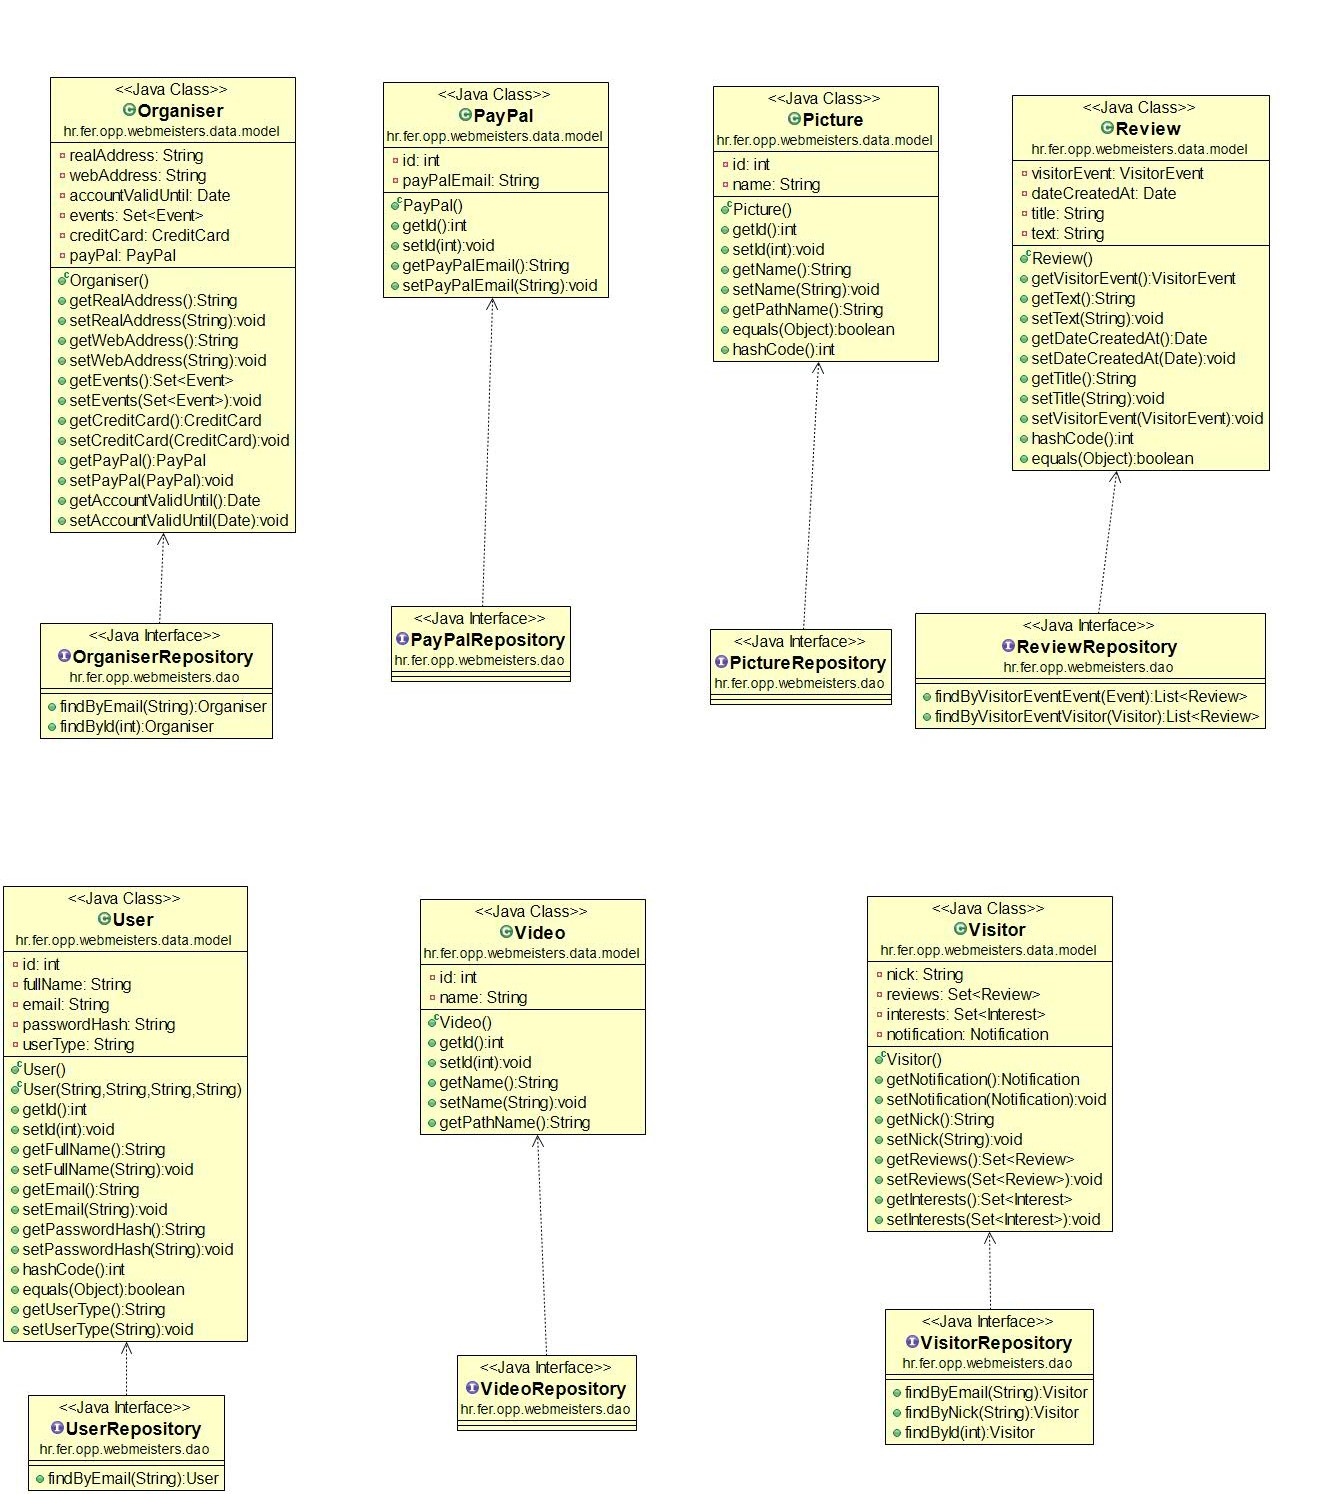
\includegraphics[scale=0.4]{slike/dijagram2a.jpg}
			\centering
			\caption{Poveznica objekta i Repositoryja}
			\label{fig:dijagramraz3}
		\end{figure}
	
		\begin{figure}[H]
			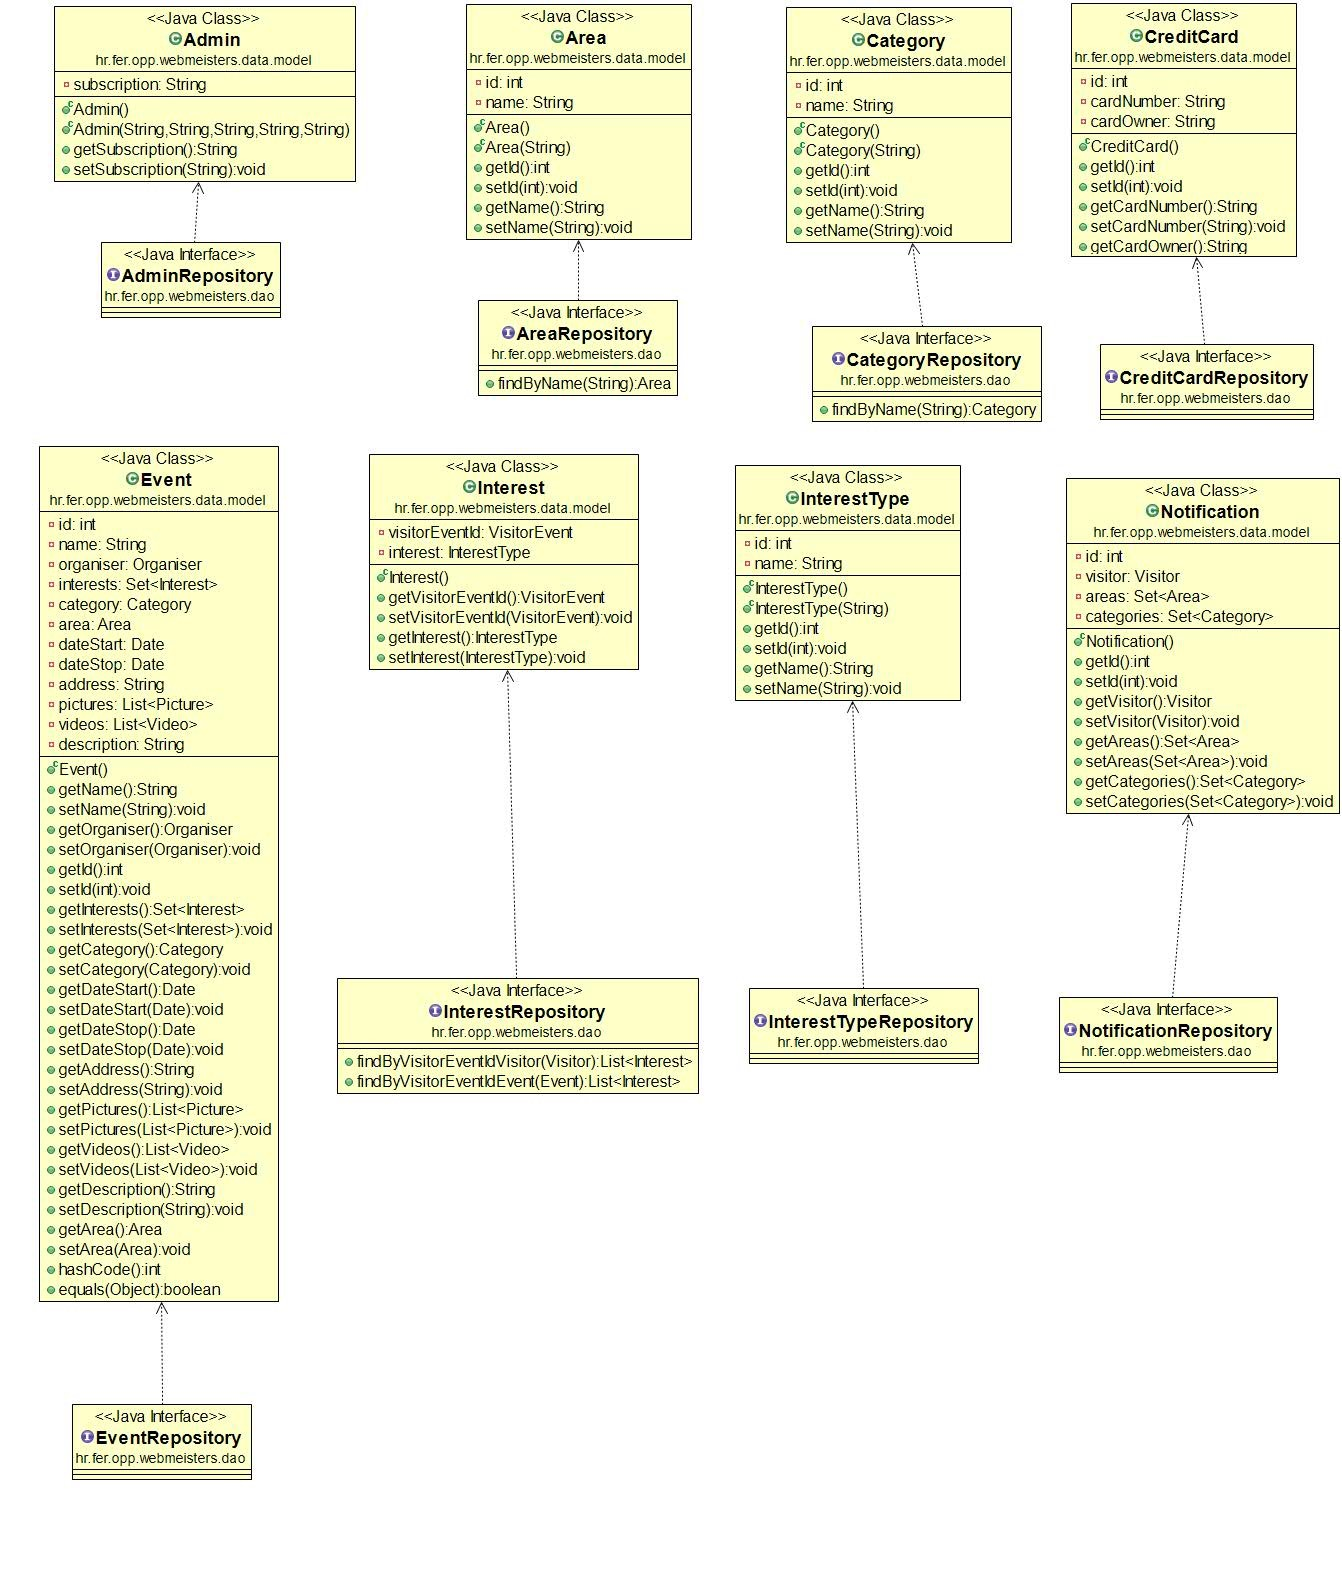
\includegraphics[scale=0.4]{slike/dijagram2b.jpg}
			\centering
			\caption{Nastavak poveznica objekta i Repositoryja}
			\label{fig:dijagramraz4}
		\end{figure}
		
		\normalfont U nastavku slijedi prikaz svih Controllera koji primaju zahtjeve, obrađuju ih i dalje zovu odgovarajuću JSP datoteku koja generira HTML sadržaj. 
		
		\normalfont\noindent Zbog kompleksne situacije nisu prikazane poveznice svakog Controllera sa svim Serviceima.
		
		\begin{figure}[H]
			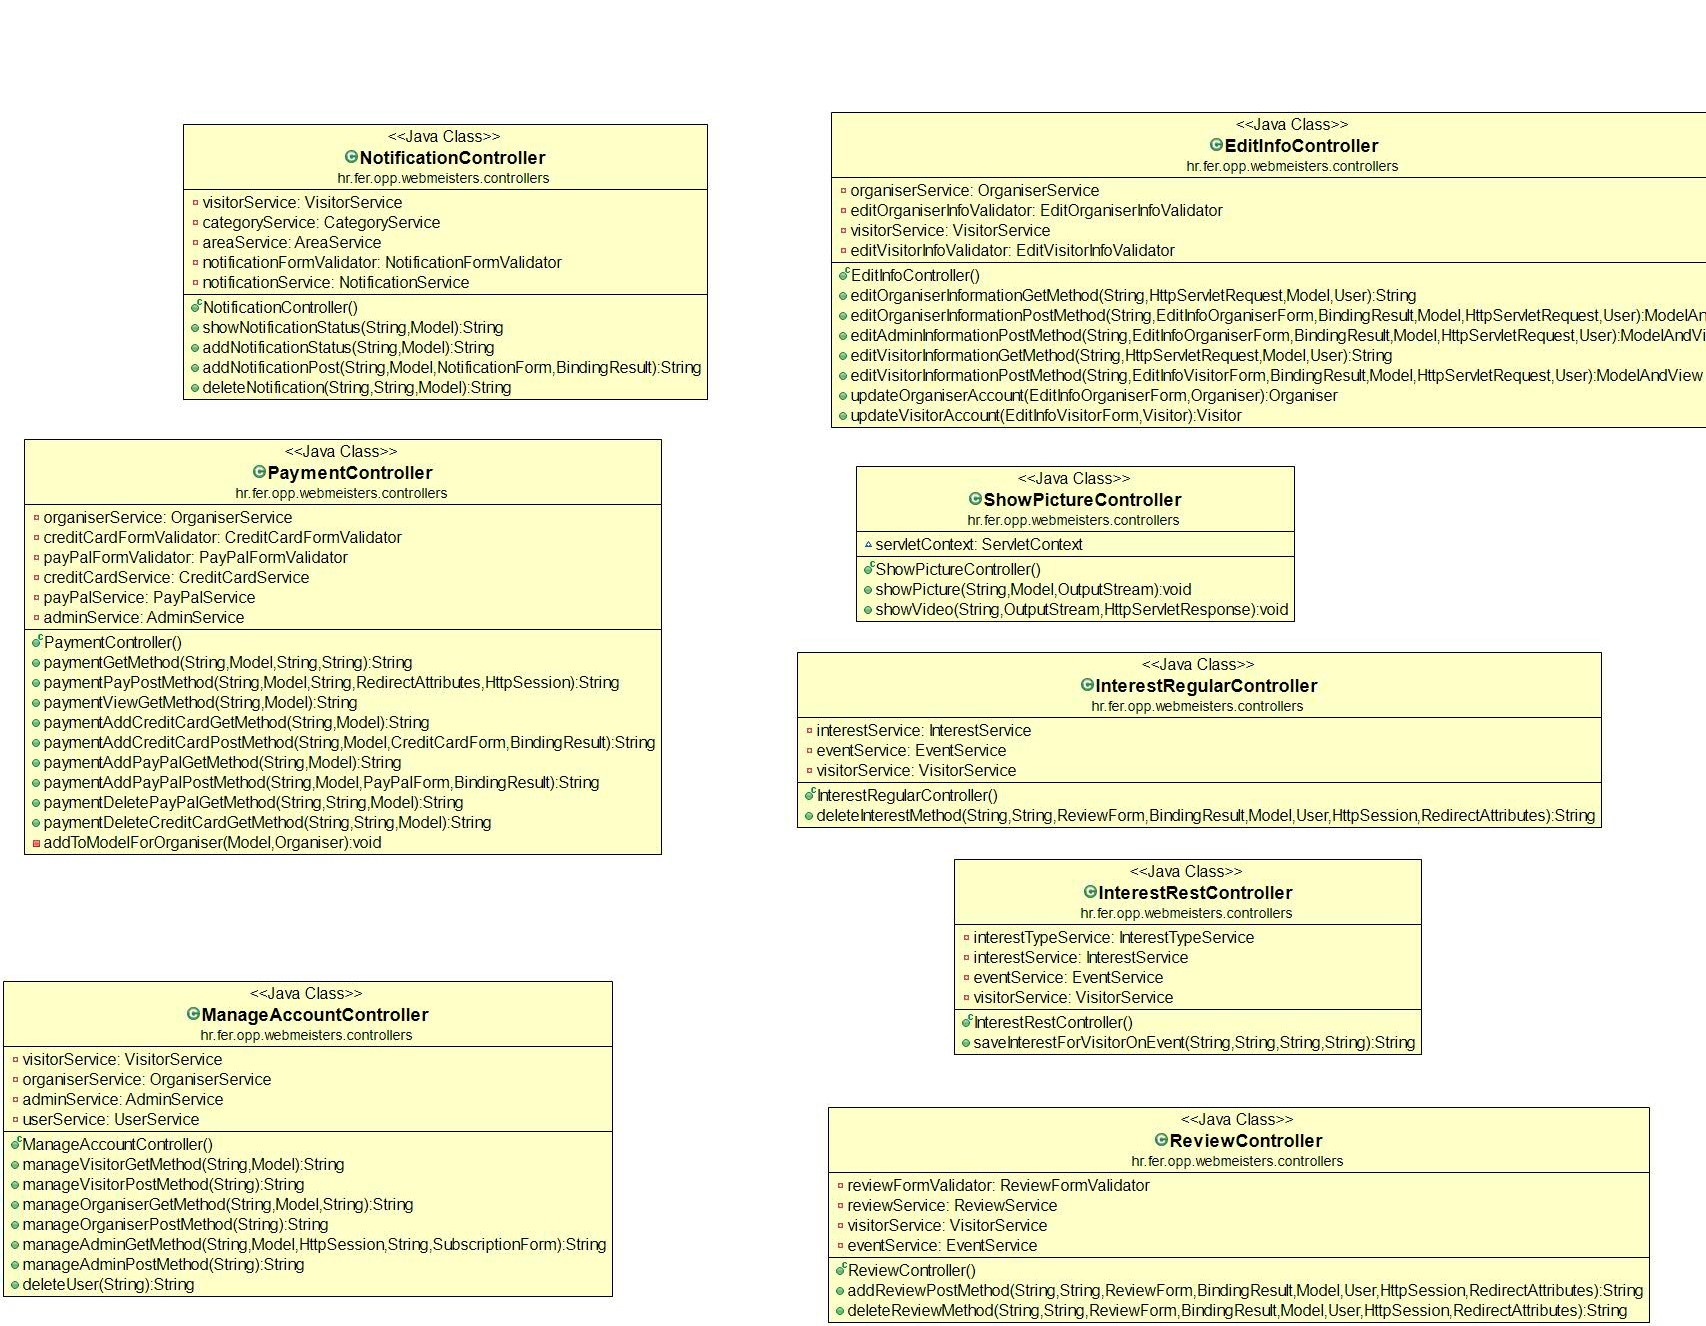
\includegraphics[scale=0.4]{slike/dijagram3a.jpg}
			\centering
			\caption{Controlleri prvi dio}
			\label{fig:dijagramraz5}
		\end{figure}
	
	\noindent\textbf{NotificationController – } služi za dodavanje notifikacija i brisanje notifikacija te prikaz notifikacija ako su postavljene\\
	\textbf{EditInfoController – } služi za uređivanje korisničkih informacija\\
	\textbf{PaymentController – } služi za plaćanje, dodavanje i brisanje kreditne kartice te dodavanje i brisanje Paypal računa kod organizatora\\
	\textbf{ShowPictureController – } služi za prikaz fotografija na web stranici\\
	\textbf{InterestRegularController, InterestRestController – } dodavanje, brisanje interesa  kod događaja\\
	\textbf{ManageAccountController – } služi za prikaz informacija svih korisnika \\
	\textbf{ReviewController – } služi za dodavanje recenzija
	
		\begin{figure}[H]
			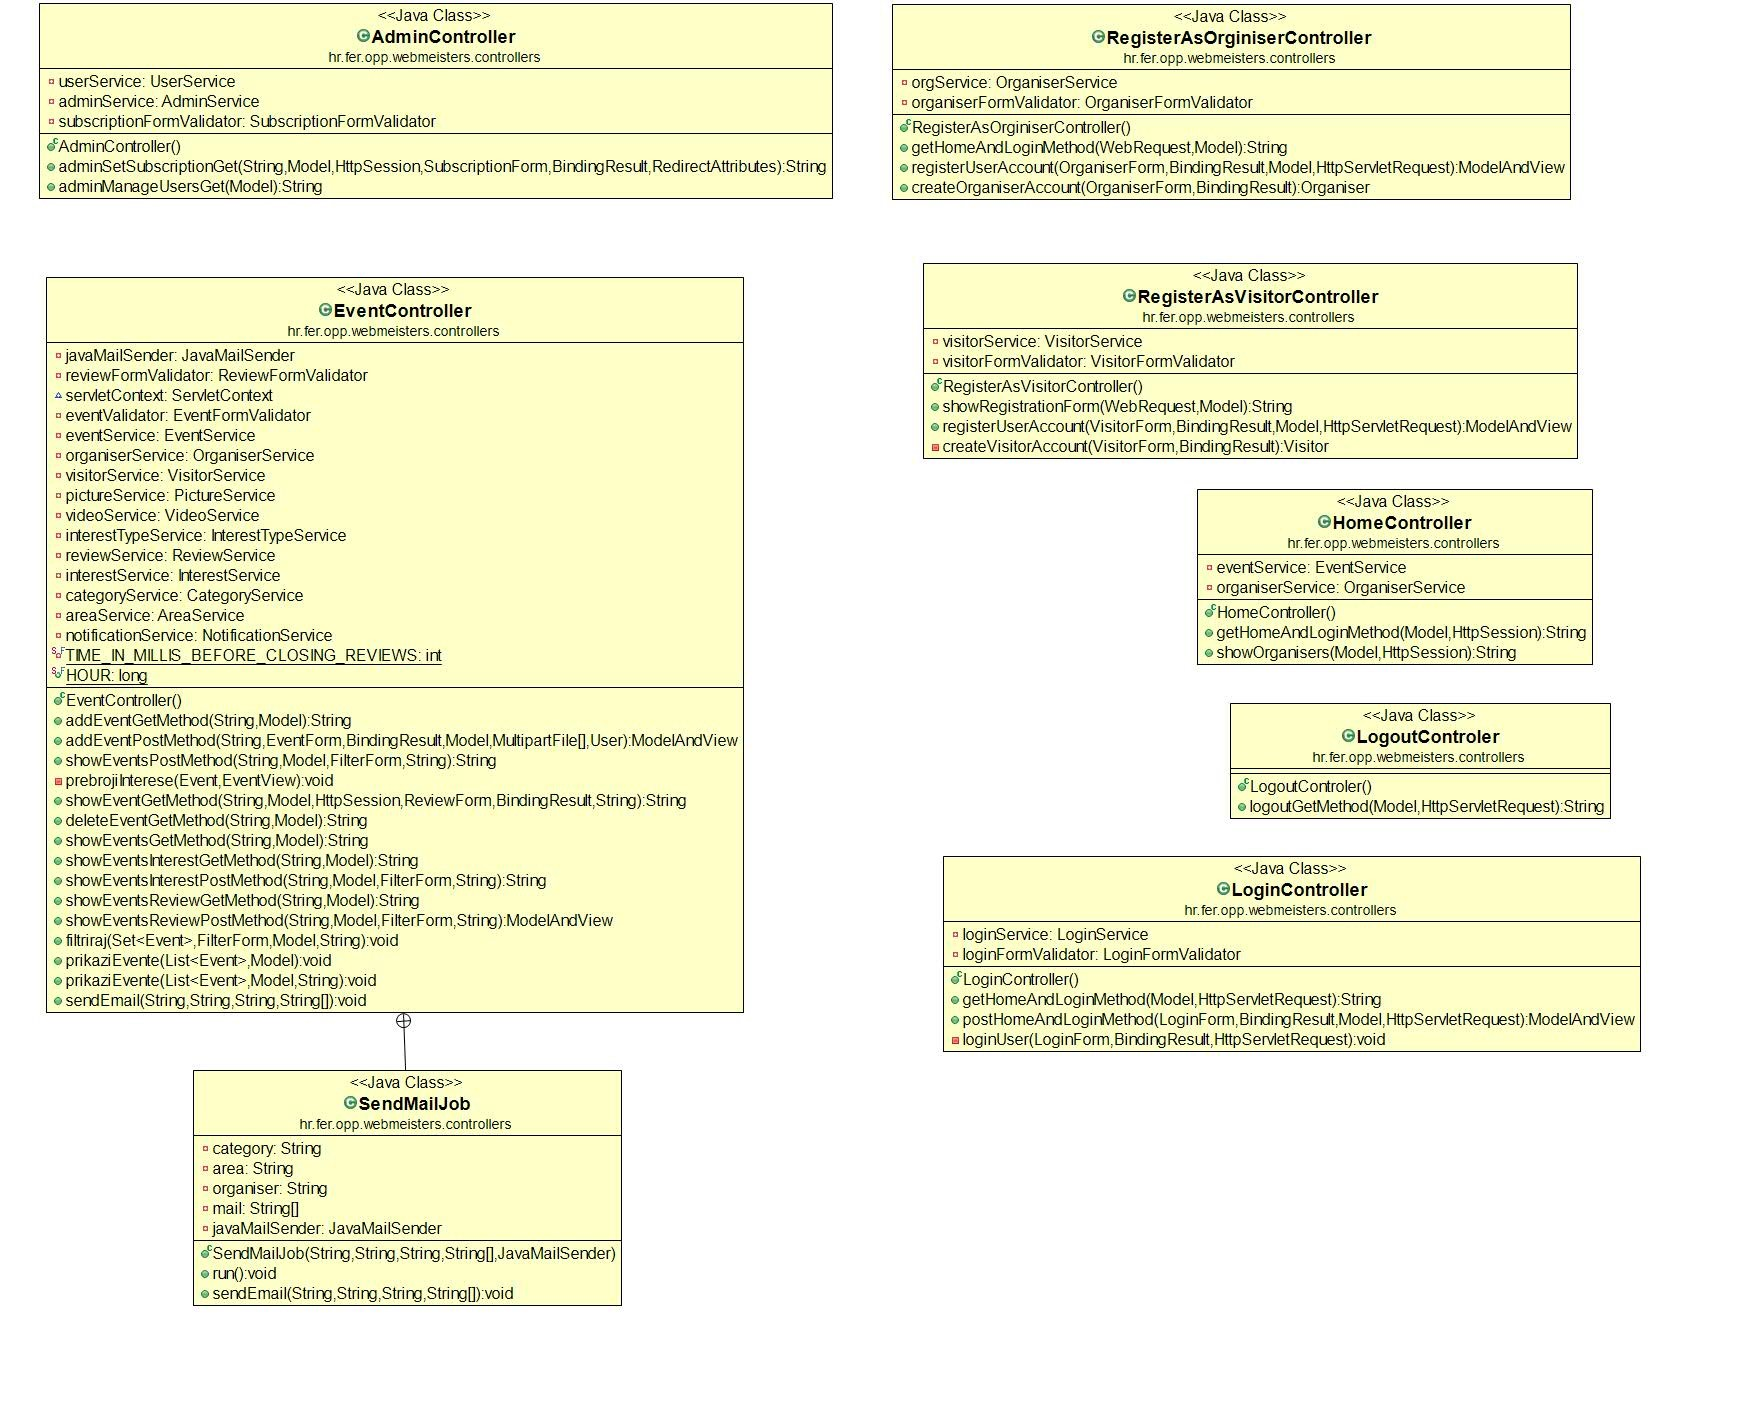
\includegraphics[scale=0.4]{slike/dijagram3b.jpg}
			\centering
			\caption{Controlleri drugi dio}
			\label{fig:dijagramraz6}
		\end{figure}
	
	\noindent\textbf{AdminController – } služi svim adminovim funkcionalnostima\\
	\textbf{RegisterAsOrganiser,RegisterAsVistior – } registracija korisnika\\
	\textbf{Login,LogoutController – } prijava i odjava korisnika\\
	\textbf{EventController – } služi za dodavanja i brisanje događaja, filtriranje događaja, slanje maila kod dodavanja događaja ako postoje postavke obavijesti za nekog korisnika, prikazivanje jednog događaja ili više njih\\
	
	\normalfont\noindent Kako bi bili sigurni da je svaki formular ispravno ispunjen, to provjeravamo na način pošaljemo Formu koja se ispuni, a odgovarajući Validator provjeri je li to dobro ispunjeno. Tek kad je ispunjeno kako treba biti, upišemo podatke u bazu.
	
		\begin{figure}[H]
			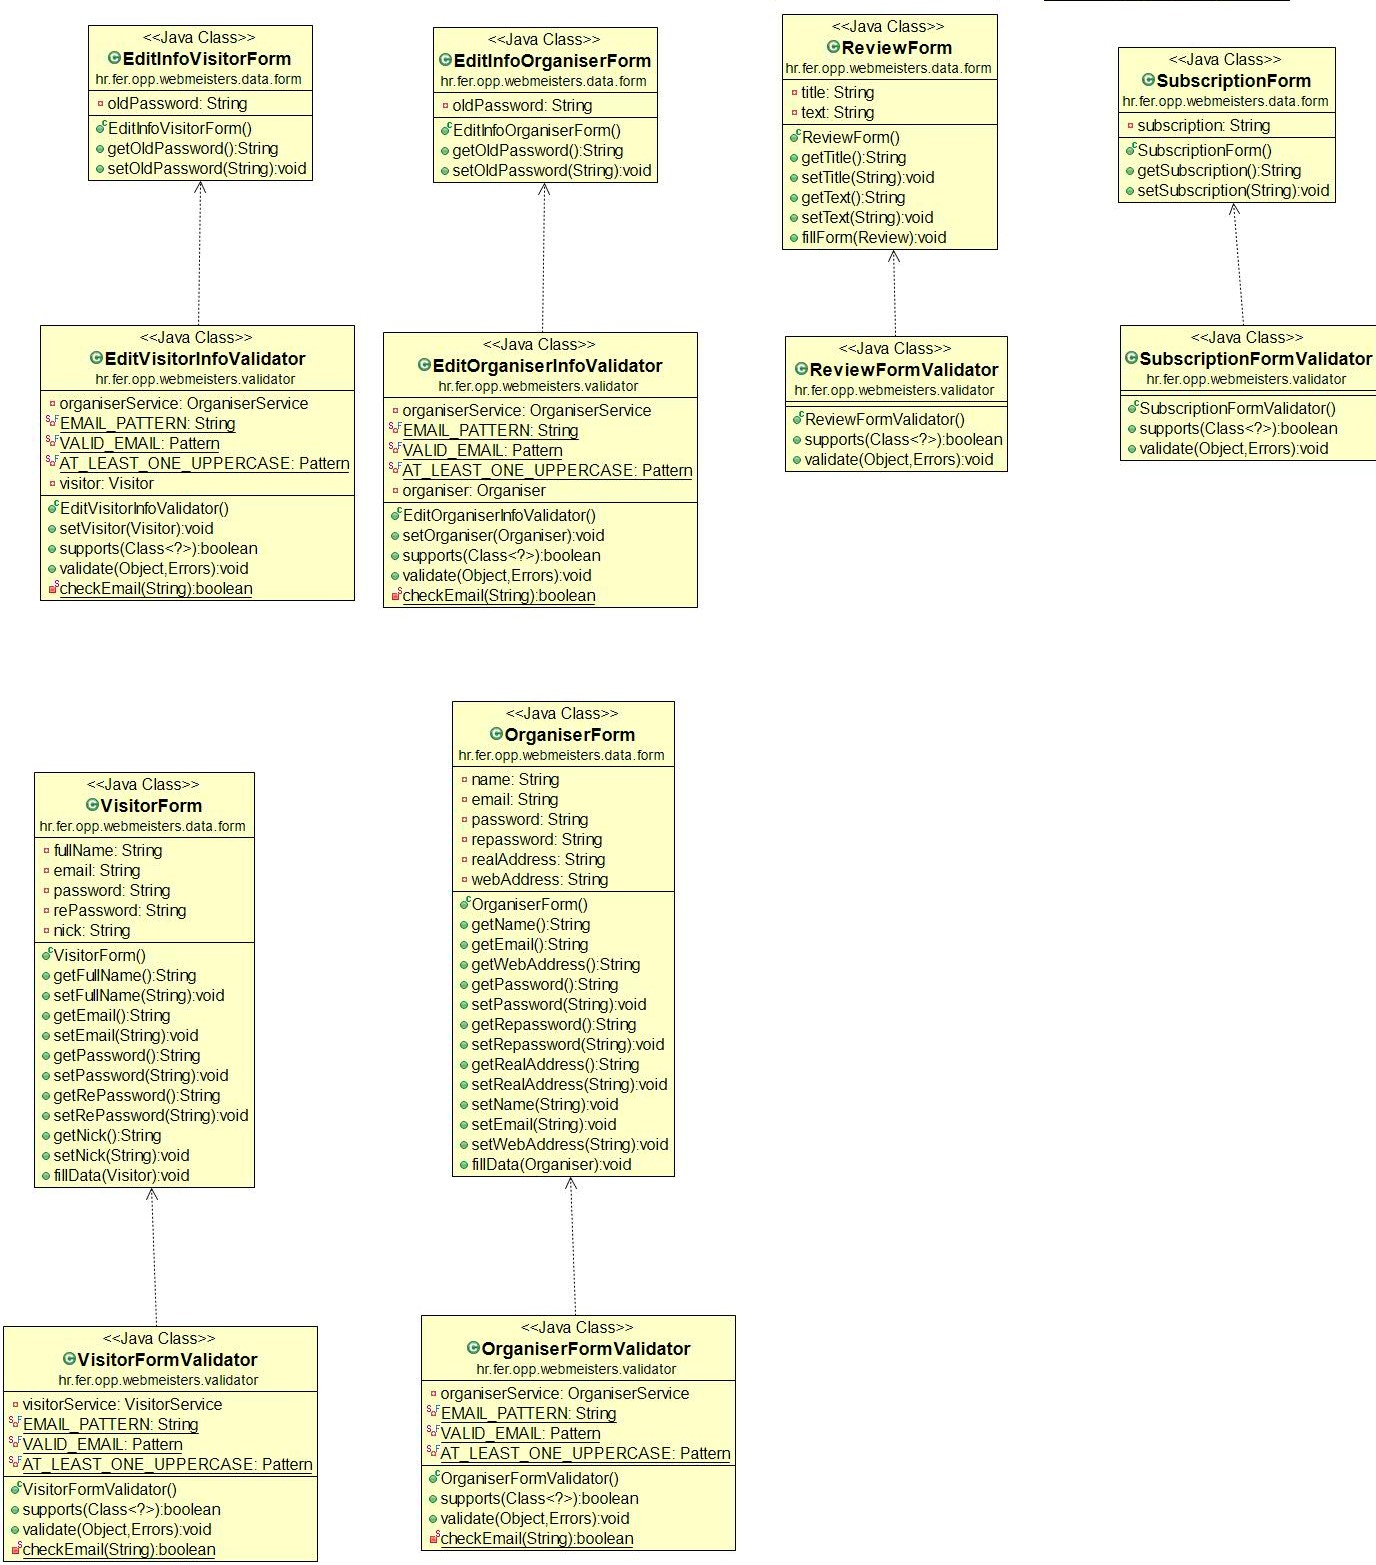
\includegraphics[scale=0.4]{slike/dijagram4a.jpg}
			\centering
			\caption{Validatori i Forme prvi dio}
			\label{fig:dijagramraz7}
		\end{figure}
	
		\begin{figure}[H]
			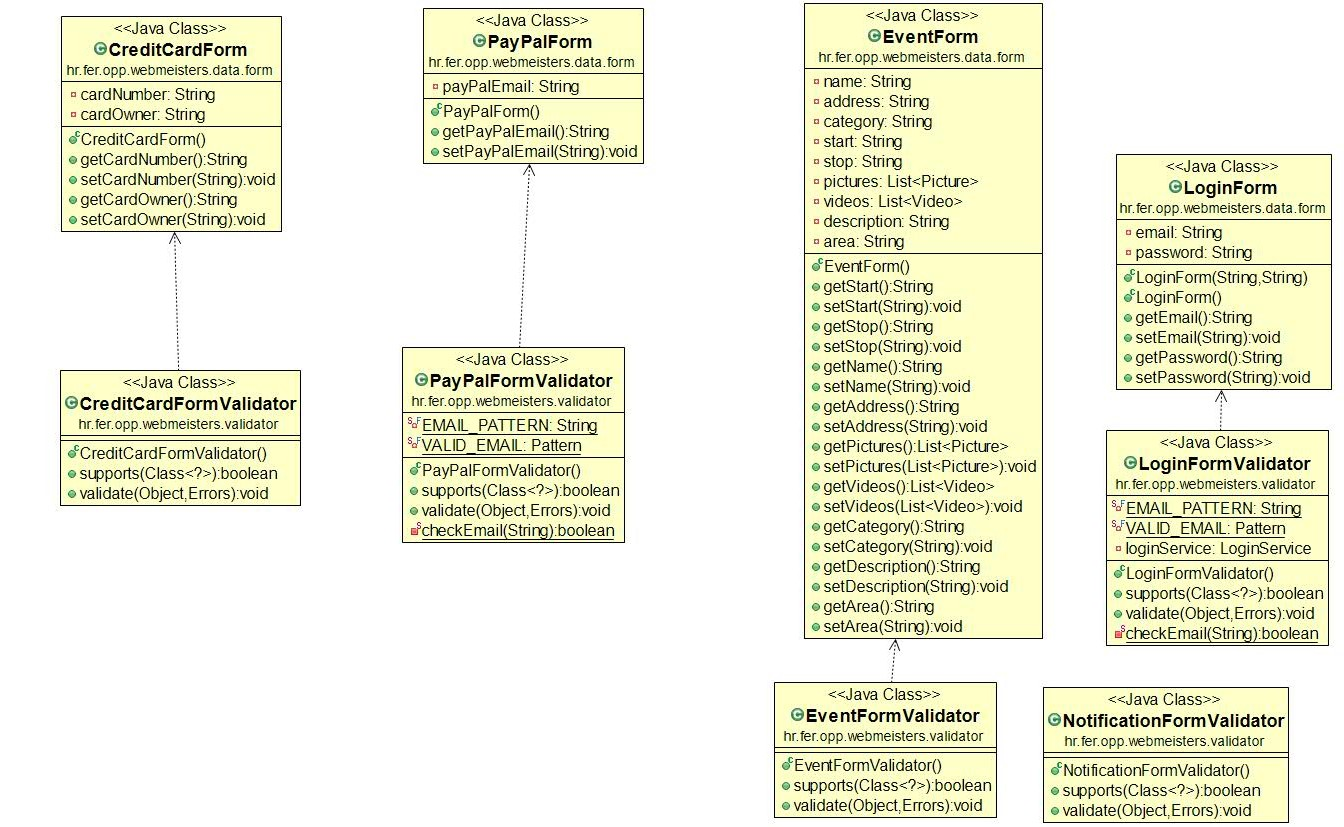
\includegraphics[scale=0.4]{slike/dijagram4b.jpg}
			\centering
			\caption{Validatori i Forme drugi dio}
			\label{fig:dijagramraz8}
		\end{figure}
	
			
		\eject
		
		\section{Dijagram stanja}
			\normalfont\noindent Dijagram stanja se koristi kao grafički prikaz prijelaz iz jednog stanja u drugo na temelju događaja.
			
			\medskip
			
			\normalfont\noindent Na slici \ref{fig:dijagramstorg} prikazan je dijagram stanja registriranog organizatora.
			
			\medskip
			
			\normalfont\noindent Nakon prijave, organizatoru se prikazuje početna stranica sa aktualnim događajima i notifikacija o plaćanju članarine ovisno jeli ona plaćena ili nije sa poveznicom koja ga vodi do plaćanja članarine.
			
			\medskip
			
			\normalfont\noindent Na vrhu web stranice nalazi se traka sa tri gumba, “Naslovnica”, “Ime profila organizatora” I “Odjavi se”, koji su vidljivi tokom cijelog rada na web aplikaciji.
			
			\medskip
			
			\normalfont\noindent Organizator pored svakog događaja može kliknuti na gumb “Više o događaju” koji ga vodi na stranicu tog događaja sa dodatnim informacijama.
			
			\medskip
			
			\normalfont\noindent Klikanjem gumba “Ime profila organizatora” otvara se profil organizatora sa svim informacijama. Organizator ima opciju uređivanja podataka profila i pregledavanja vlastitih događaja.
			
			\medskip
			
			\normalfont\noindent Također ima opciju i plaćanja članarine kojom se otvara nova stranica na kojoj unosi načine plaćanja, Paypal ili karticu, te odabire način plaćanja i plaća članarinu.
			
			\medskip
			
			\normalfont\noindent Ukoliko je članarina plaćena organizatoru se prikazuje gumb “Dodaj događaj” kojim može dodavati nove događaje što uključuje dodavanje opisa događaja, odabir kategorije događaja, mjesto održavanja te različiti medijski sadržaji uključujući video zapise i slike.
			
			\medskip
			
			\normalfont\noindent Također ako je članarina plaćena organizator u pregledavanju vlastitih događaja ima opciju i brisanja događaja.
			
			\medskip
			
			\begin{figure}[H]
				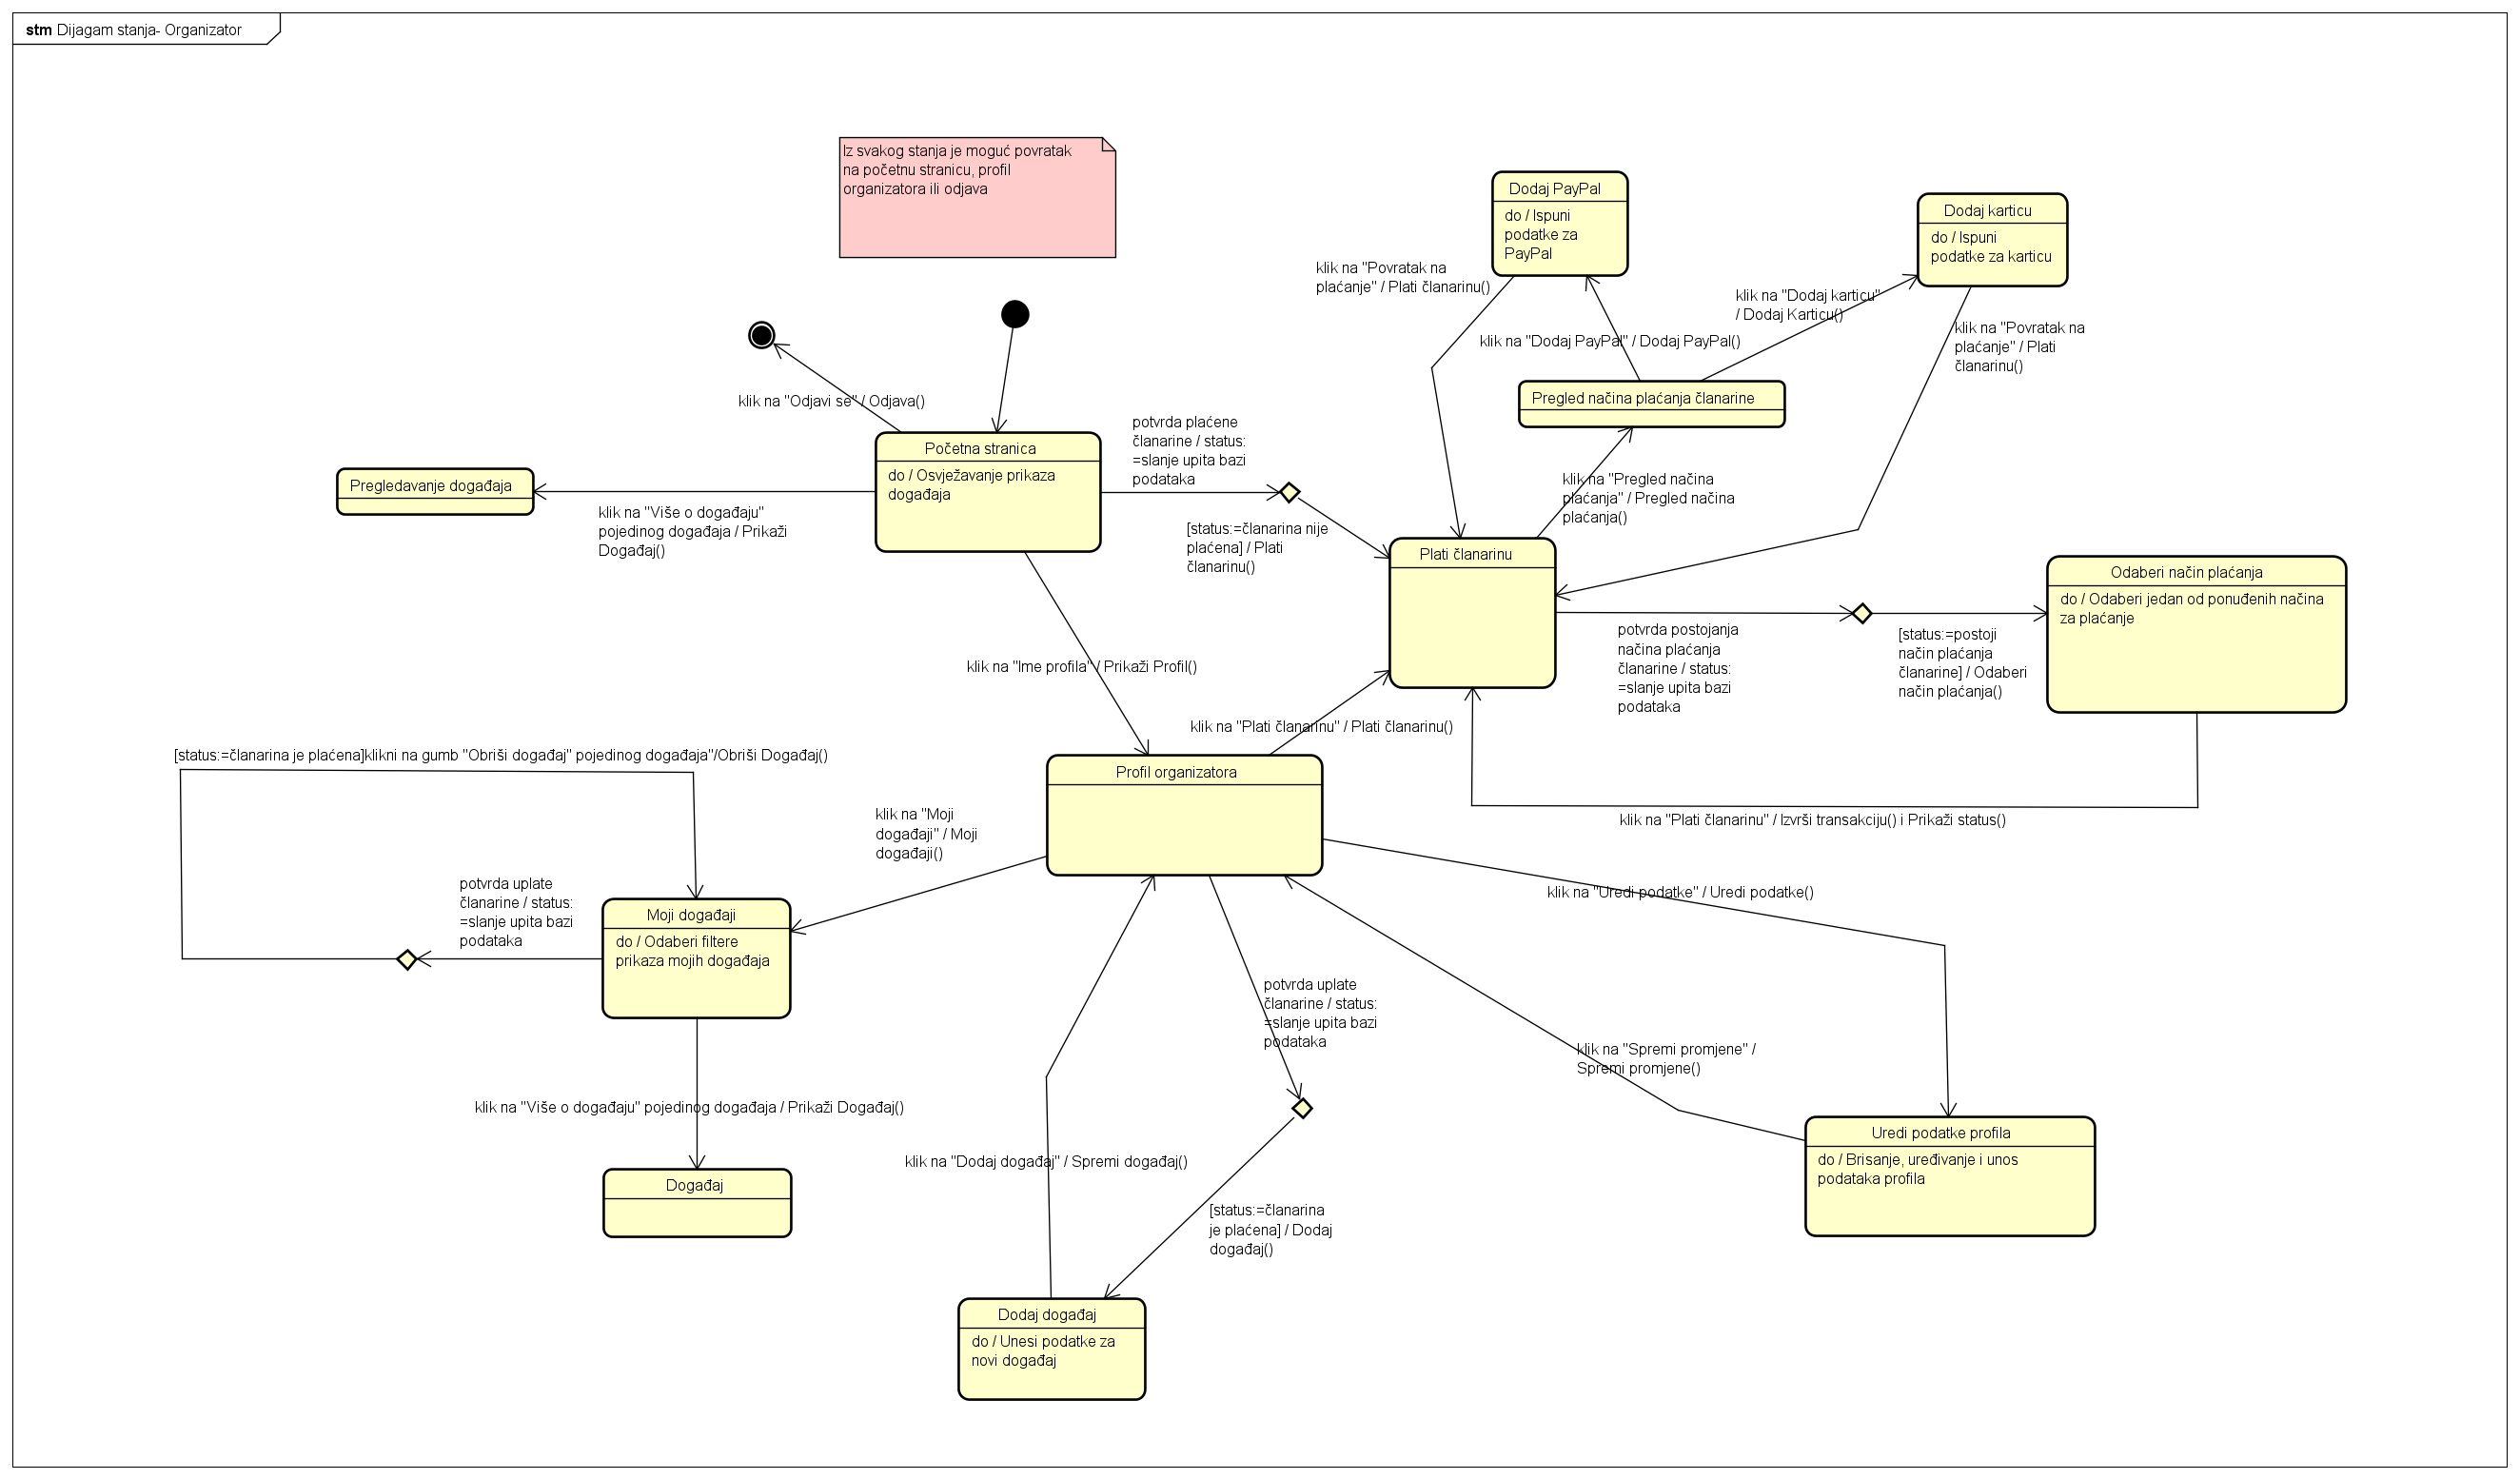
\includegraphics[width=\linewidth]{slike/dijagram_stanja.PNG}
				\centering
				\caption{Dijagram stanja - Organizator}
				\label{fig:dijagramst}
			\end{figure}
			
			\bigskip
			
			
			\eject 
		
		\section{Dijagram aktivnosti}
		
		\normalfont Dijagram na slici prikazuje slijedne aktivnosti koje rezultiraju dodavanjem recenzije za neko događanje. Preduvjet za dodavanje recenzije je taj da prijavljeni korisnik bude posjetitelj. Nakon što se korisnik prijavi kao posjetitelj prikaže mu se početna stranica na kojoj se nalazi popis događanja. Potom posjetitelj odabere događanje za koje želi dodati svoju recenziju te, ukoliko je događanje završilo unutar posljednjih 48h i posjetitelj nije već dodao svoju recenziju za njega, prilikom prikaza detalja o događanju posjetitelju će biti prikazana i opcija dodavanja recenzije. Ukoliko barem jedan od ta dva uvjeta nije zadovoljen posjetitelju neće biti prikazana opcija za dodavanje recenzije već će mu pisati prikladna poruka o nemogućnosti recenziranja. Po završetku pisanja teksta svoje recenzije posjetitelj odabirom opcije za spremanje označi kraj željene akcije te se njegova recenzija pohrani u bazu podataka i prikaže na ekranu. 
		
				\begin{figure}[H]
					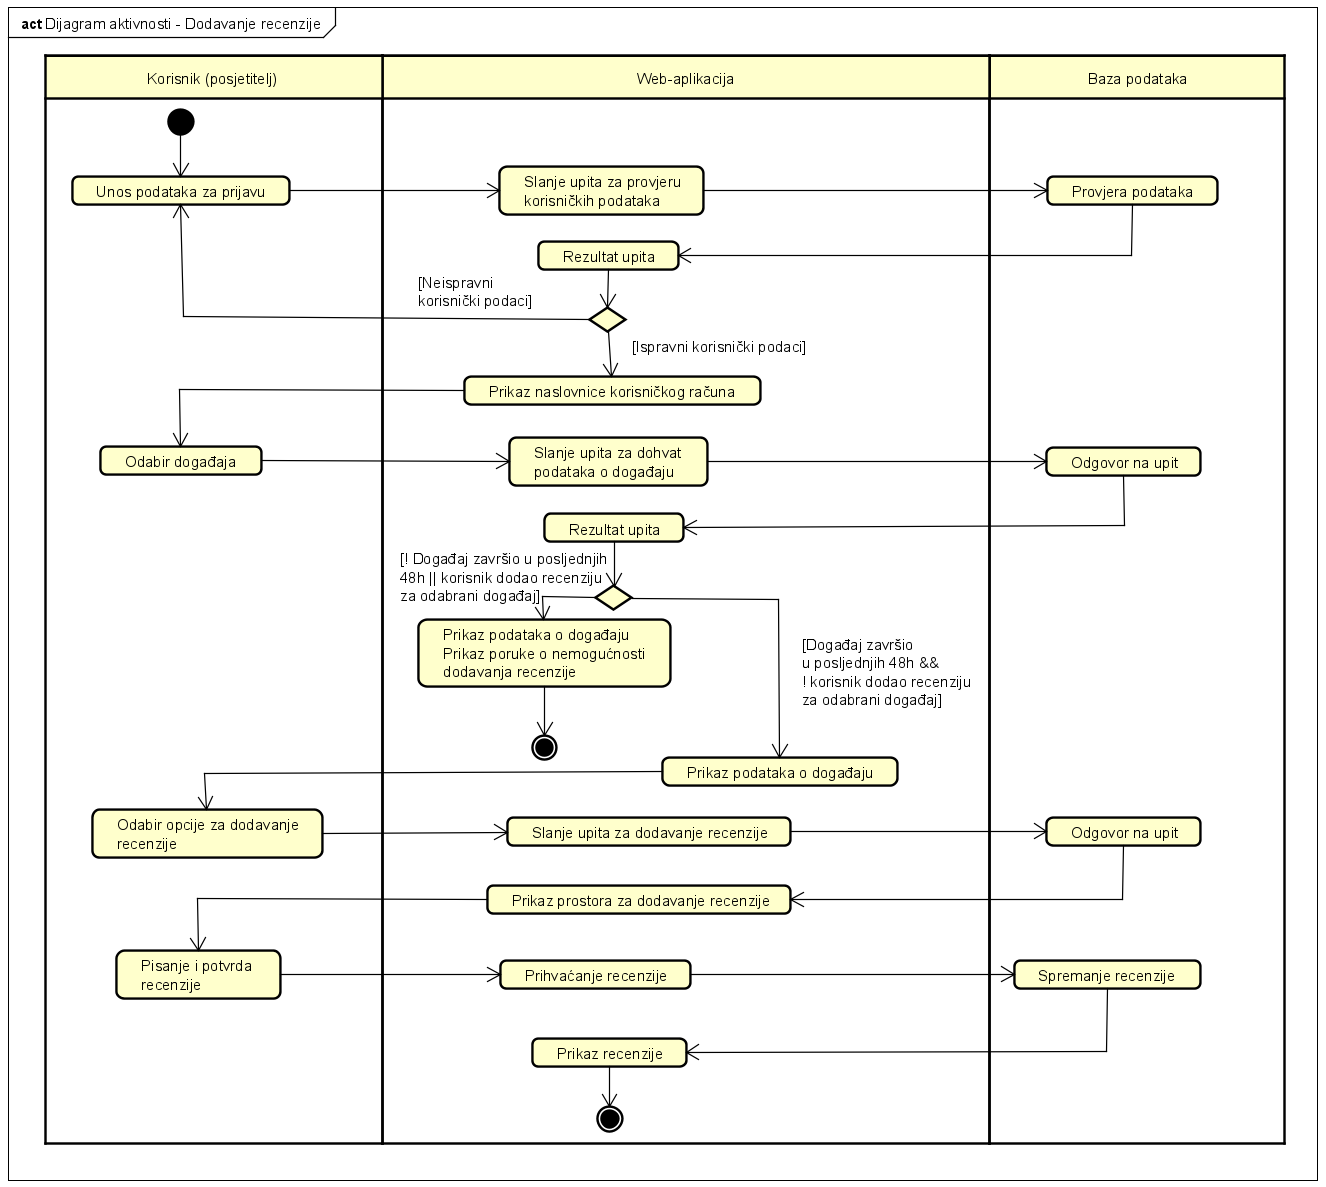
\includegraphics[width=\linewidth]{slike/dijagram_akrivnosti.PNG}
					\centering
					\caption{Dijagram aktivnosti - Dodavanje recenzije}
					\label{fig:dijagram}
				\end{figure}
			
			\eject
		
		\section{Dijagram komponenti}
		
		\normalfont Dijagram komponenti prikazan na slici 4.9  opisuje organizaciju komponenti, međuovisnosti i odnose prema okolini. Sustavu se pristupa preko dva sučelja. Preko sučelja za dohvat JSP datoteka u kojima je html kod i CSS datoteka se poslužuju datoteke koje pripadaju frontend dijelu aplikacije. Korisnik komunicira sa web aplikacijom pomoću JSP view komponenata te ovisno o korisnikovim akcijama osvježava prikaz i dohvaća nove podatke ili datoteke. Controller komponente u REST sloju komuniciraju sa Service komponentama u REST sloju, a zadaća Service komponenti jest usklađivanje i „uljepšavanje“ podataka iz baze (SQL upiti) s podacima iz Controllera (forme modela). Za dohvat podataka iz baze koristi se JpaRepository koji se spaja na bazu. 
		
		\begin{figure}[H]
			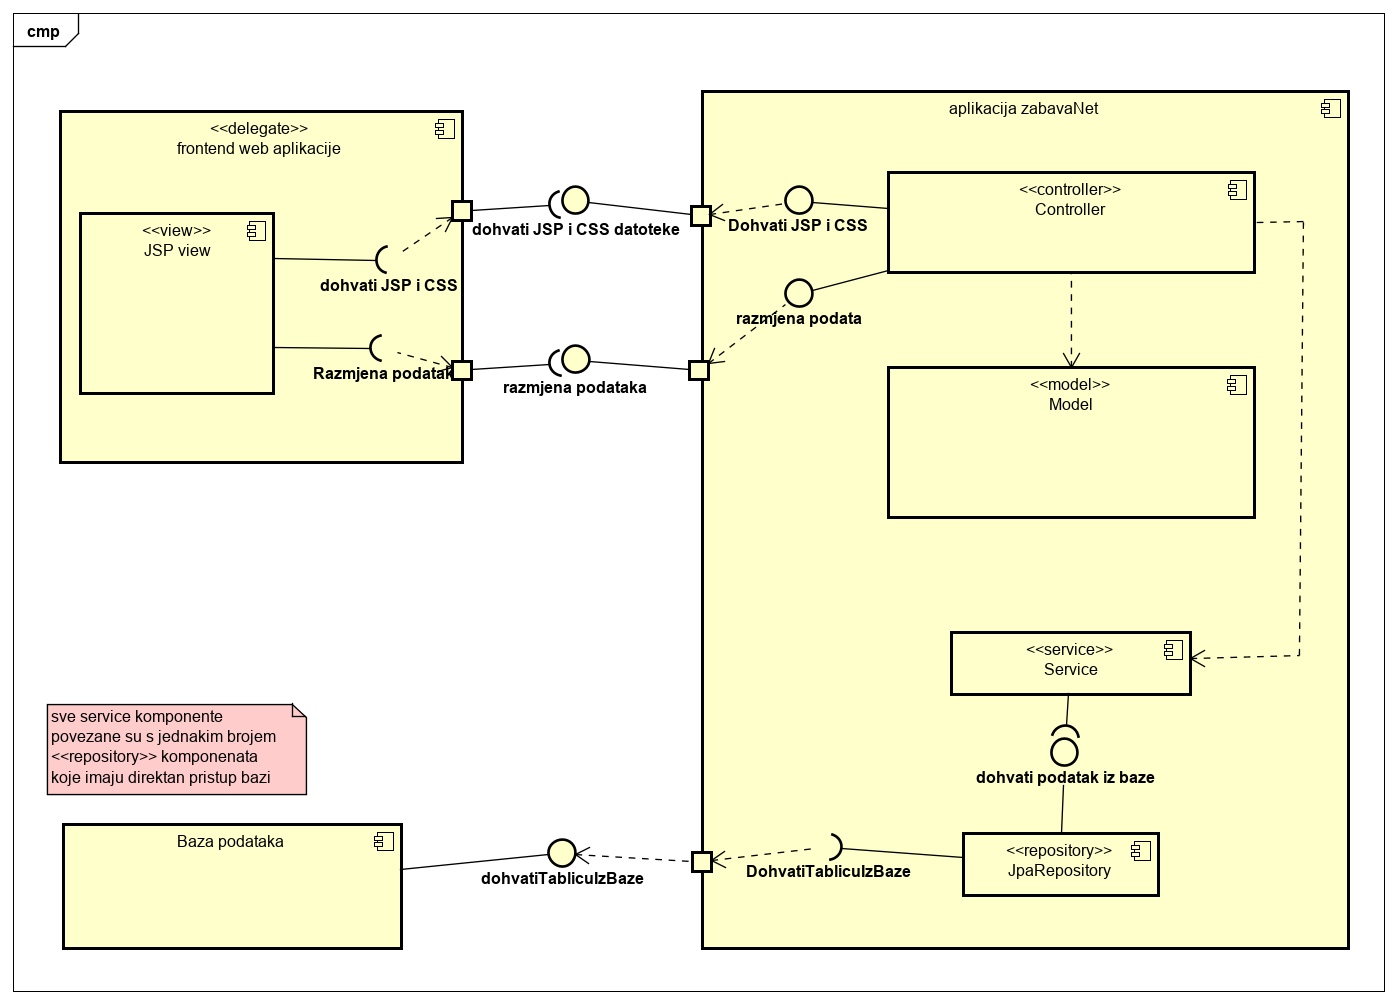
\includegraphics[width=\linewidth]{slike/dijagram_komponenti.PNG}
			\centering
			\caption{Dijagram komponenti}
			\label{fig:dijagramkomp}
		\end{figure}
		
		
